\documentclass[twoside,11pt]{article}

\usepackage{blindtext}

% Any additional packages needed should be included after jmlr2e.
% Note that jmlr2e.sty includes epsfig, amssymb, natbib and graphicx,
% and defines many common macros, such as 'proof' and 'example'.
%
% It also sets the bibliographystyle to plainnat; for more information on
% natbib citation styles, see the natbib documentation, a copy of which
% is archived at http://www.jmlr.org/format/natbib.pdf

% Available options for package jmlr2e are:
%
%   - abbrvbib : use abbrvnat for the bibliography style
%   - nohyperref : do not load the hyperref package
%   - preprint : remove JMLR specific information from the template,
%         useful for example for posting to preprint servers.
%
% Example of using the package with custom options:
%
% \usepackage[abbrvbib, preprint]{jmlr2e}

\usepackage{jmlr2e}

% Definitions of handy macros can go here

\newcommand{\dataset}{{\cal D}}
\newcommand{\fracpartial}[2]{\frac{\partial #1}{\partial  #2}}

% Heading arguments are {volume}{year}{pages}{date submitted}{date published}{paper id}{author-full-names}

\usepackage{lastpage}
\usepackage{tabularx}
\usepackage{amsmath}
\usepackage{amsfonts}
\usepackage{booktabs}
\usepackage{longtable}
\usepackage{listings}
\renewcommand{\lstlistingname}{}
\PassOptionsToPackage{table}{xcolor}
\usepackage{xcolor}
\usepackage{booktabs}
\usepackage{multirow}
\usepackage{xcolor}

\usepackage{dirtree}

% \usepackage{geometry}
\usepackage{hyperref}
\usepackage{colortbl}
\usepackage[most]{tcolorbox}

% Required packages in the preamble:
\usepackage{booktabs}
\usepackage[table]{xcolor}
\usepackage{pifont}
\usepackage{colortbl}
\usepackage{graphicx}

% =========================================================
% Packages Required
% =========================================================
\usepackage[most]{tcolorbox}
\usepackage{tabularx}
\usepackage{booktabs}
\usepackage{array}
\usepackage{enumitem}
\usepackage[table]{xcolor}
\usepackage{tikz}
\usetikzlibrary{shadows.blur, positioning}

% --------------------------------------------------
% Colors and Boxes
% --------------------------------------------------
\usepackage[dvipsnames]{xcolor}
\usepackage[most]{tcolorbox}
\tcbuselibrary{skins,breakable,listings}

% --------------------------------------------------
% Code Listings
% --------------------------------------------------
\usepackage{listings}

% --------------------------------------------------
% Better Lists
% --------------------------------------------------
\usepackage{enumitem}

% =========================================================
% Custom Colors
% =========================================================
\definecolor{MainBlue}{RGB}{32,74,135}
\definecolor{SoftBlue}{RGB}{239,245,255}
\definecolor{LineBlue}{RGB}{88,126,191}
\definecolor{AccentBlue}{RGB}{15,52,96}


\newcommand{\cmark}{\textcolor{green!70!black}{\ding{51}}}
\newcommand{\xmark}{\textcolor{red!75!black}{\ding{55}}}


\tcbset{
    colback=blue!5,
    colframe=blue!60!black,
    fonttitle=\bfseries,
    coltitle=black
}


\newtcolorbox{scalabilitynote}{
  colback=green!5,
  colframe=green!50!black,
  colbacktitle=green!15,
  coltitle=black,
  fonttitle=\bfseries,
  title=Scalability Note
}

\newcommand{\pmark}{\textcolor{orange!80!black}{$\circ$}}




\definecolor{codegreen}{rgb}{0,0.6,0}
\definecolor{codegray}{rgb}{0.5,0.5,0.5}
\definecolor{codepurple}{rgb}{0.58,0,0.82}
\definecolor{backcolour}{rgb}{0.95,0.95,0.92}

\lstdefinestyle{mystyle}{
    backgroundcolor=\color{backcolour},   
    commentstyle=\color{codegreen},
    keywordstyle=\color{magenta},
    numberstyle=\tiny\color{codegray},
    stringstyle=\color{codepurple},
    basicstyle=\ttfamily\footnotesize,
    breakatwhitespace=false,         
    breaklines=true,                 
    captionpos=b,                    
    keepspaces=true,                 
    numbers=left,                    
    numbersep=5pt,                  
    showspaces=false,                
    showstringspaces=false,
    showtabs=false,                  
    tabsize=2
}


% --------------------------------------------------
% Python Listing Style
% --------------------------------------------------
\lstdefinestyle{pythonstyle}{
    language=Python,
    basicstyle=\ttfamily\small,
    keywordstyle=\color{blue},
    commentstyle=\color{ForestGreen},
    stringstyle=\color{BrickRed},
    backgroundcolor=\color{gray!8},
    frame=single,
    rulecolor=\color{black!20},
    breaklines=true,
    showstringspaces=false,
    tabsize=4
}

% --------------------------------------------------
% Bash Listing Style
% --------------------------------------------------
\lstdefinestyle{bashstyle}{
    language=bash,
    basicstyle=\ttfamily\small,
    backgroundcolor=\color{gray!8},
    frame=single,
    rulecolor=\color{black!20},
    breaklines=true,
    showstringspaces=false
}

\newtcolorbox{testingstats}{
    enhanced,
    breakable,
    colback=blue!3,
    colframe=blue!70!black,
    coltitle=black,
    title=Testing Statistics,
    fonttitle=\bfseries,
    boxrule=0.8pt,
    arc=2mm,
    left=3mm,
    right=3mm,
    top=2mm,
    bottom=2mm,
    drop shadow
}

\lstset{style=mystyle}
\jmlrheading{1}{2026}{1-\pageref{LastPage}}{X/26}{X/26}{XX-XXXX}{Rezaee, Ziabakhsh, Bahrampour, Ghoreishi, Khajeh, Sajedifar, Chalak, Zerafatangiz and Eskandari}
\ShortHeadings{SCPP: A Python Library for Soft Clustering}{Rezaee et al.}
\firstpageno{1}

\begin{document}

\title{SCPP: A Unified Python Library for Soft Clustering}


\author{%
\name Kiyan Rezaee \email kiyanrezaee17@gmail.com \\
\name Morteza Ziabakhsh \email morteza24mail@protonmail.com \\
\name Artin Bahrampour \email Artinbahrampour1599@gmail.com \\
\name Seyed Mohammad Ghoreishi \email mohammad.ghoreishi530@gmail.com \\
\name Asal Khajeh \email Asalkhajeh1@gmail.com \\
\name Ali Sajedifar \email Its.AliSajedifar@gmail.com \\
\name Manny Chalak \email manee.ch83@gmail.com \\
\name Ava Zerafatangiz \email ava.zerafattt@gmail.com \\
\name Sadegh Eskandari \email eskandari@guilan.ac.ir  \\
\addr Department of Computer Science, University of Guilan, Rasht, Iran%
}

\editor{}

\maketitle

\begin{abstract}
Soft clustering methods are distributed across Python packages with
inconsistent estimator interfaces, parameter conventions, and membership
representations, making systematic comparison across methodological families
difficult. We present \textbf{SCPP} (\textbf{\underline{S}oft
\underline{C}lustering \underline{P}ython \underline{P}ackage}), an
open-source Python library that collects 42 soft clustering algorithms
spanning fuzzy, possibilistic, evidential, probabilistic, graph-based,
matrix-factorization, ensemble, and deep-learning approaches behind a common
estimator protocol. SCPP does not standardize what an algorithm consumes ---
inputs are irreducibly heterogeneous --- but it does standardize everything
after the fit call: every estimator exposes soft cluster assignments through
a membership matrix $U \in \mathbb{R}^{n \times K}_{\geq 0}$, together with
labels, prototypes and cluster count of consistent shape and semantics. A
conformance suite fits all 42 estimators and checks that contract in
continuous integration. The library ships an evaluation framework with 20
datasets and 12 cluster-validity metrics, and we use it for the cross-family
comparison the protocol makes possible: all 20 feature-matrix estimators over
the full dataset suite under one protocol, with every failure reported rather
than dropped. Where an independent implementation of the same algorithm
exists, we check against it: SCPP's fuzzy c-means agrees with
\texttt{scikit-fuzzy} to $6.2\times10^{-10}$ and its Gaussian mixture with
\texttt{scikit-learn} to $1.0\times10^{-12}$, with identical hard partitions.
We additionally report an implementation optimization study in which
profiling identified bottlenecks in five implementations; rewriting them
reduced runtime by a median of $70\times$ relative to SCPP's own
pre-optimization code across 20 paired measurements, with a maximum of
$4{,}507\times$, while remaining numerically indistinguishable from the
preserved references (maximum membership difference $2.2\times10^{-14}$ across
42 comparisons). SCPP is documented, tested with 1{,}183 automated tests
across 48 modules at 95\% line coverage, integrated with continuous
integration across three operating systems and four Python versions, and
distributed through PyPI under the MIT license.
\end{abstract}


\begin{keywords}
soft clustering, fuzzy clustering, overlapping community detection,
Python, open-source software
\end{keywords}

\section{Introduction}

Soft clustering assigns each observation a vector of memberships over clusters rather than a single label. This is useful when observations can reasonably belong to more than one group: genes can participate in several biological pathways, documents can cover multiple topics, network nodes can belong to overlapping communities, and software classes can have cross-cutting responsibilities \citep{dogan2025fuzzy,liu2025llm,cangemi2025fuzzy,chi2025novel,ziabakhsh2025extracting,rezaee2025fos}.

Despite the breadth of soft clustering methods, their software support is
partitioned by family rather than by task. Within a family the tooling is
often good. \texttt{scikit-fuzzy} \citep{scikit_fuzzy_2024},
\texttt{fuzzy-c-means} \citep{dias2019fuzzy} and \texttt{fuzzycat}
\citep{oliver_fuzzycat} cover fuzzy c-means and close variants;
\texttt{scikit-learn} \citep{pedregosa2011scikit} and \texttt{Mixture-Models}
\citep{kasa2024mixture} cover probabilistic mixtures; \texttt{ClustPy}
\citep{leiber2023benchmarking} covers deep clustering with its own
benchmarking harness; and for graphs, \texttt{CDlib}
\citep{rossetti2019cdlib} exposes a large collection of community-detection
algorithms --- including overlapping ones --- behind a common
\texttt{NodeClustering} abstraction with a dedicated fuzzy variant, while
\texttt{karateclub} \citep{rozemberczki2020karateclub} provides
BigCLAM, DANMF, Ego-Splitting, M-NMF and NNSED under one scikit-learn-style
API.

We therefore do not claim that unification is itself novel: three of these
packages already unify a family. What none of them does is span families.
A study that wants to place a possibilistic method, an evidential method, a
mixed-membership blockmodel and a deep modularity network side by side must
install four ecosystems, reconcile four conventions for specifying the number
of clusters, and write its own adapter for each way of exposing a membership
matrix --- if the method exposes one at all. That integration cost is what
SCPP removes, and cross-family breadth behind one checked contract is what we
offer that the alternatives in Table~\ref{tab:comparison} do not.

The problem is not that different algorithms need different inputs; that
difference is real and cannot be abstracted away. A prototype method needs a
feature matrix, a community detection method needs a graph, a consensus
method needs a set of partitions. The problem is that their \emph{outputs}
are also represented differently, for no reason intrinsic to the methods.
\textbf{SCPP (\underline{S}oft \underline{C}lustering \underline{P}ython
\underline{P}ackage)} draws exactly that line: algorithm-specific inputs and
internal optimization are left alone, while every estimator's fitted state
and evaluation workflow follow one interface.

Our contributions are summarized as follows:

\begin{enumerate}[leftmargin=*,topsep=2pt,itemsep=1pt]

\item \textbf{A common estimator protocol, checked rather than asserted.}
All SCPP estimators implement \texttt{fit} and expose standardized attributes
--- \texttt{memberships\_}, \texttt{labels\_}, \texttt{centers\_} and
\texttt{n\_clusters} --- with consistent shapes and semantics. A conformance
suite constructs and fits \emph{all 42} exported estimators and verifies the
contract on every commit; an estimator the suite cannot construct fails CI
(\S\ref{sec:design}, \S\ref{sec:quality}).

\item \textbf{Cross-family coverage.}
SCPP provides 42 algorithms spanning fuzzy, possibilistic, evidential,
probabilistic, graph-based, matrix-factorization, document, ensemble and deep
soft clustering (Table~\ref{tab:comparison}, Appendix~\ref{app:algorithms}).
Twelve of them are, to our knowledge, without an independently maintained
Python implementation.

\item \textbf{Evaluation, exercised rather than shipped.}
SCPP provides 20 datasets, 12 cluster-validity metrics and tools for runtime,
memory and scalability measurement. We use them: Appendix~\ref{app:performance}
reports all 20 feature-matrix estimators over the full dataset suite --- 220
fits under one protocol, with the 32 that timed out, ran out of memory or
returned a degenerate partition reported as such.

\item \textbf{Validation against independent implementations.}
Where a third-party implementation of the same algorithm exists, we check
against it rather than only against ourselves. SCPP's fuzzy c-means matches
\texttt{scikit-fuzzy} to $6.2\times10^{-10}$ and its Gaussian mixture matches
\texttt{scikit-learn} to $1.0\times10^{-12}$, with identical hard partitions
at every size tested (Appendix~\ref{app:external}).

\item \textbf{An implementation optimization study.}
Profiling under a common protocol identified concrete bottlenecks in five
implementations. Rewriting them reduced runtime by a median of $70\times$
relative to SCPP's own pre-optimization code, with a maximum of
$4{,}507\times$, verified against preserved references
(\S\ref{sec:benchmark}, Appendix~\ref{app:optimization}).

\item \textbf{Reproducible software infrastructure.}
1{,}183 automated tests at 95\% line coverage, CI across three operating
systems and four Python versions, published documentation, 42 runnable
examples, and distribution under the MIT license (\S\ref{sec:quality}).

\end{enumerate}




\begin{table}[t]
\centering
\footnotesize
\setlength{\tabcolsep}{4pt}
\definecolor{headerbg}{RGB}{232,245,233}
\definecolor{scppbg}{RGB}{220,252,231}
\definecolor{altrow}{RGB}{248,250,252}
\renewcommand{\arraystretch}{1.15}

\caption{\textbf{Python packages providing soft clustering methods.}
\emph{Soft methods} counts estimators that expose a per-sample membership,
responsibility or affiliation matrix through the package's public API; the
same rule is applied to every row including ours, so \texttt{scikit-learn}
counts \texttt{GaussianMixture}, \texttt{BayesianGaussianMixture},
\texttt{LatentDirichletAllocation} and \texttt{NMF}. Counts were taken from
each package's public API in August 2026 and are approximate for the two
large graph libraries, whose algorithm sets change between releases.
\cmark~= supported, \pmark~= partial, \xmark~= not provided.
\emph{Checked API} means the package ships a test that fits every exported
estimator and asserts a documented output contract, rather than documenting
one.}
\label{tab:comparison}

\begin{tabular}{lrcccccc}
\toprule
\textbf{Package}
& \textbf{Soft}
& \textbf{Fuzzy}
& \textbf{Prob.}
& \textbf{Graph}
& \textbf{Deep}
& \textbf{Checked}
& \textbf{Benchmarking} \\
& \textbf{methods}
&
&
&
&
& \textbf{API}
& \\
\midrule

\texttt{fuzzy-c-means}~\citep{dias2019fuzzy}
& 1 & \cmark & \xmark & \xmark & \xmark & \xmark & \xmark \\

\texttt{fuzzycat}~\citep{oliver_fuzzycat}
& 1 & \cmark & \xmark & \xmark & \xmark & \xmark & \xmark \\

\texttt{scikit-fuzzy}~\citep{scikit_fuzzy_2024}
& 1 & \cmark & \xmark & \xmark & \xmark & \xmark & \xmark \\

\texttt{HDBSCAN}~\citep{mcinnes2017hdbscan}
& 1 & \xmark & \pmark & \xmark & \xmark & \xmark & \xmark \\

\texttt{pyclustering}~\citep{novikov2019pyclustering}
& 2 & \cmark & \pmark & \xmark & \xmark & \xmark & \xmark \\

\texttt{scikit-learn}~\citep{pedregosa2011scikit}
& 4 & \xmark & \cmark & \xmark & \xmark & \cmark & \pmark \\

\texttt{ClustPy}~\citep{leiber2023benchmarking}
& 6 & \pmark & \cmark & \xmark & \cmark & \xmark & \cmark \\

\texttt{Mixture-Models}~\citep{kasa2024mixture}
& 8 & \xmark & \cmark & \xmark & \xmark & \xmark & \xmark \\

\texttt{karateclub}~\citep{rozemberczki2020karateclub}
& $\sim$5 & \xmark & \xmark & \cmark & \pmark & \xmark & \xmark \\

\texttt{CDlib}~\citep{rossetti2019cdlib}
& $\sim$15 & \pmark & \xmark & \cmark & \pmark & \xmark & \cmark \\

\midrule
\rowcolor{scppbg}
\textbf{SCPP (this work)}
& \textbf{42}
& \cmark
& \cmark
& \cmark
& \cmark
& \cmark
& \cmark \\

\bottomrule
\end{tabular}
\end{table}




%=========================================================================
\section{Design and Implementation}
\label{sec:design}

\paragraph{What is standardized, and what is not.}
SCPP does not force different algorithms to accept the same input. Prototype
methods take a feature matrix, graph methods an adjacency or affinity matrix,
consensus methods a set of partitions, document methods raw text; the first
argument of \texttt{fit} is whatever the algorithm actually needs, and
Appendix~\ref{app:algorithms} lists the input modality of every estimator.
What SCPP standardizes is the fitted state. Every estimator accepts its
parameters through \texttt{\_\_init\_\_}, \texttt{fit} returns \texttt{self},
and \texttt{memberships\_} is an $(n, K)$ matrix with non-negative entries;
\texttt{labels\_} is its row-wise $\arg\max$, and \texttt{centers\_} is
provided when the method has prototypes.

\paragraph{What the protocol does not promise.}
Two limits are worth stating plainly, because a protocol that looks like
scikit-learn's invites assumptions it does not meet. First, most soft
clustering algorithms are \emph{transductive}: they partition the data they
were fitted on and define no rule for assigning an unseen sample. Calling
\texttt{predict()} with no argument returns the fitted partition; passing new
data raises \texttt{NotImplementedError} rather than silently returning the
training labels, which would be a partition of different data with the wrong
length. Only \texttt{SoftKSC} defines a genuine out-of-sample rule. Second,
estimators implement \texttt{get\_params} and \texttt{set\_params}, so
\texttt{sklearn.base.clone} and parameter introspection work, but they are
\emph{not} drop-in scikit-learn clusterers: \texttt{fit} signatures differ by
modality and no estimator defines \texttt{score}, so tools requiring a
uniform \texttt{fit(X, y)} or a default scorer do not apply.

\paragraph{Implementation.}
The interface is implemented through a single \texttt{BaseSoftClusterer}
class, which wraps each subclass's own entry point and normalises the result
afterwards. Adding an existing algorithm therefore does not require rewriting
it or changing its call signature. Each algorithm lives in its own module
under \texttt{soft\_clustering/} with a reference to its original
publication. Estimators are imported lazily, so \texttt{import
soft\_clustering} pulls in nothing a user does not touch; the core
installation is NumPy, SciPy, scikit-learn and \texttt{typeguard}. The four
PyTorch-backed models (CDCGS, DMoN, NOCD, RDFKC) sit behind the \texttt{deep}
extra and raise an explicit installation message when it is absent. A CI job
installs the built wheel into a clean environment and imports and constructs
every estimator, so this claim is checked rather than described.

\begin{lstlisting}[language=Python, caption={Fitting an estimator (FCM) and reading its soft output.}]
from sklearn.datasets import load_iris
from soft_clustering import FCM

X, y = load_iris(return_X_y=True)
model = FCM(n_clusters=3, m=2.0, random_state=0).fit(X)
U = model.memberships_        # (150, 3), rows sum to 1
centers = model.centers_      # (3, 4)
labels = model.labels_        # (150,), argmax over U
\end{lstlisting}


\paragraph{Implementation performance.}
Collecting the algorithms behind one interface also makes their computational
cost measurable under one protocol. We audit every implementation the same
way: all 42 are checked statically for loop structure and numerical call
sites, the 30 the shared harness can construct are baseline-timed at
$n = 200$, and the 10 slowest are profiled at the function level. Fifteen
complete a 200-sample fit in under $10$\,ms with the numerical work already
delegated to NumPy or SciPy, and were left unchanged. For five, profiling
identified a specific bottleneck --- most often a scalar operation invoked
inside a Python loop where a batched equivalent existed. Those five were
reworked and compared against preserved copies of the originals; a speedup is
reported only where the rewrite produces equivalent results, and the same
equivalence checks run in CI. We do not claim the remaining implementations
are optimal, only that measurement did not identify a change worth making.
Appendix~\ref{app:optimization} gives the protocol, the five cases and the
measurements, and is explicit that the baseline is SCPP's own earlier code;
Appendix~\ref{app:external} is the comparison against third-party
implementations.

\paragraph{Extension.}
Adding a new algorithm to SCPP requires only implementing the algorithm-specific
training procedure and returning its membership matrix through the common
interface. The base class \texttt{BaseSoftClusterer} automatically provides shared functionality, including
cluster labels, prediction methods, and consistent handling of the number of
clusters. After registering the estimator, the conformance suite verifies that
it follows the required protocol, and the new method becomes immediately
available to the existing evaluation and benchmarking tools without additional
integration code.

%=========================================================================
\section{Evaluation and Benchmarking}
\label{sec:benchmark}

\paragraph{Datasets.} \texttt{benchmarking.datasets} returns a standardised
$(X, y)$ pair for 20 datasets in three groups: five bundled with
scikit-learn (iris, wine, digits, breast cancer, olivetti faces), six
synthetic generators with controlled overlap and anisotropy, and nine fetched
from OpenML ($n$ from 214 to 20{,}000, $K$ from 4 to 26). Ground-truth labels
are used only for external validation. The OpenML group is downloaded on
first use and is therefore the one part of the suite that depends on network
access and on OpenML's continued availability; the eleven bundled and
generated datasets are fully offline and are what the results in
Appendix~\ref{app:performance} use.

\paragraph{Metrics.} \texttt{soft\_clustering\_metrics} computes seven
measures on $U$ --- partition coefficient, modified partition coefficient,
partition entropy, fuzzy hypervolume, Xie--Beni index, fuzzy compactness and
fuzzy separation --- and \texttt{clustering\_metrics} computes five on
defuzzified labels (silhouette, Calinski--Harabasz, Davies--Bouldin, ARI,
NMI). Entropies use the natural logarithm. Two properties of this module
matter for interpreting any table built from it, and are enforced in code
rather than left to the reader (Appendix~\ref{app:metrics}): the first three
indices measure how \emph{crisp} a partition is rather than how good it is,
and they are undefined unless the rows of $U$ sum to one, so they are
reported as \texttt{nan} for possibilistic and affiliation-based methods
instead of as a number on a different scale.

\paragraph{Computational measurement.}
\texttt{RuntimeBenchmark}, \texttt{MemoryBenchmark} and
\texttt{ScalabilityBenchmark} measure fit and prediction time, resident
memory, and their scaling with dataset size; \texttt{ClusteringBenchmark}
runs a set of estimators across a set of datasets and returns a
\texttt{pandas} DataFrame. \texttt{RuntimeBenchmark} takes a warm-up fit and
reports the minimum over repetitions by default, matching the protocol of
Appendix~\ref{app:optimization}, because a mean over cold runs is dominated
by first-call overhead.

\paragraph{What we measure with it.}
Appendix~\ref{app:performance} reports the cross-family comparison: all 20
estimators that consume a feature matrix, over all 11 offline datasets, 220
fits under one protocol. Appendix~\ref{app:external} reports agreement and
runtime against third-party implementations of the same algorithms. Both are
regenerated from the repository by a single command.

%=========================================================================
\section{Software Quality, Documentation, and Availability}
\label{sec:quality}

\paragraph{Testing.}
The suite contains 1{,}183 tests across 48 modules and achieves 95\% line
coverage. Each algorithm has method-specific tests; on top of those sit four
cross-cutting suites. The \emph{conformance suite} constructs and fits all 42
exported estimators and checks the protocol: \texttt{fit} returns
\texttt{self}; \texttt{memberships\_} has shape $(n, K)$ and is non-negative;
estimators that impose the partition constraint produce rows summing to one;
\texttt{labels\_} equals $\arg\max U$; \texttt{predict()} fails before
fitting; \texttt{predict(X)} either works or raises rather than returning the
training labels; \texttt{get\_params} round-trips through
\texttt{sklearn.clone}; and a fixed \texttt{random\_state} reproduces the
memberships. It is tied to the public registry, so adding an estimator
without a conformance entry fails CI --- and, unlike an earlier revision, the
suite permits no exclusions at all. An \emph{honesty check} guards the
partition-constraint declaration in the other direction: an estimator may not
declare that it does not normalise while normalising unconditionally, because
that silently disables the check for itself. The \emph{edge-case suite}
covers duplicate and coincident points, singular covariances, $K > n$,
$K = 1$, fuzzifiers near 1 and near infinity, \texttt{float32} input,
non-C-contiguous input, non-finite input, and empty and complete graphs,
under one rule: an estimator must either produce a valid partition or raise.
The \emph{agreement suite} compares estimators against third-party
implementations (Appendix~\ref{app:external}).

We are explicit about what this does and does not establish. Line coverage
measures which statements execute, not whether the right thing is computed:
these suites verify output contracts, invariants, recovery of planted
structure, and --- for the four algorithms where an independent
implementation exists --- numerical agreement with it. For the other 38, the
evidence is invariants and planted-structure recovery, which is weaker.

\paragraph{Continuous integration.} GitHub Actions runs the suite on Ubuntu,
macOS and Windows for Python 3.10--3.13, the full twelve-way cross-product.
Four further jobs guard claims made in this paper: one installs the built
wheel into a clean environment and imports and constructs every estimator,
then fits one estimator from each input modality; one executes all 42 example
scripts; one regenerates every count quoted here with
\texttt{tools/paper\_stats.py}; and one runs \texttt{ruff} and
\texttt{black}. Coverage is reported to Codecov on every pull request, and
Dependabot opens monthly dependency updates.

\paragraph{Documentation.} Installation instructions, per-algorithm API
reference and runnable examples are published at
\url{https://soft-clustering.readthedocs.io} and rebuilt in CI. The
repository carries 42 standalone example scripts, one per algorithm, a
contributing guide, a code of conduct, a changelog, and issue templates.

\paragraph{Availability.} SCPP is released under the MIT license, developed
in the open at \url{https://github.com/soft-clustering/soft-clustering}, and
installed with \texttt{pip install soft-clustering} (or
\texttt{soft-clustering[deep]} for the PyTorch models,
\texttt{soft-clustering[bench]} to run the benchmarking suite). All results
in this paper are regenerated from the repository by the commands listed in
Appendices~\ref{app:performance}, \ref{app:external} and
\ref{app:optimization}.

% % % % Acknowledgements and Disclosure of Funding should go at the end, before appendices and references

% % % % \acks{All acknowledgements go at the end of the paper before appendices and references.
% % % % Moreover, you are required to declare funding (financial activities supporting the
% % % % submitted work) and competing interests (related financial activities outside the submitted work).
% % % % More information about this disclosure can be found on the JMLR website.}

% % % % Manual newpage inserted to improve layout of sample file - not
% % % % needed in general before appendices/bibliography.



\newpage


\appendix


% =========================================================
% Beautiful Appendix Overview / Table of Contents
% =========================================================

\begin{tcolorbox}[
    enhanced,
    breakable,
    colback=white,
    colframe=MainBlue,
    coltitle=white,
    colbacktitle=MainBlue,
    fonttitle=\bfseries\Large,
    title={Appendix Overview},
    arc=4mm,
    boxrule=1pt,
    left=6mm,
    right=6mm,
    top=5mm,
    bottom=5mm,
    attach boxed title to top center={yshift=-2mm},
    boxed title style={
        enhanced,
        arc=3mm,
        boxrule=0pt,
        colback=MainBlue,
    },
    drop fuzzy shadow,
    before skip=12pt,
    after skip=12pt
]

% ---------------------------------------------------------
% Header Description
% ---------------------------------------------------------

\begin{center}
{\Large\bfseries\textcolor{AccentBlue}{
Supplementary Material for the SCPP}}
\end{center}

\vspace{0.8em}

% ---------------------------------------------------------
% Table Formatting
% ---------------------------------------------------------

\renewcommand{\arraystretch}{1.7}

\begin{tabularx}{\textwidth}{
    >{\centering\arraybackslash\bfseries\color{MainBlue}}m{1.2cm}
    >{\raggedright\arraybackslash}X
    >{\centering\arraybackslash\bfseries\color{MainBlue}}m{2cm}
}

\toprule

\rowcolor{SoftBlue}

\Large\textbf{Sec.}
&
\centering\arraybackslash\Large\textbf{Content}
&
\Large\textbf{Page}
\\

\midrule


\rowcolor{gray!3}

% =========================================================
% Appendix B
% =========================================================

\rowcolor{gray!3}

\Large\textbf{A}
&
\large\bfseries Implemented Algorithms in SCPP
&
\Large\pageref{app:algorithms}
\\

% =========================================================
% Appendix C
% =========================================================

\rowcolor{blue!1}

\Large\textbf{B}
&
\large\bfseries Benchmark Dataset Collection
&
\Large\pageref{app:dataset}
\\

% =========================================================
% Appendix D
% =========================================================

\rowcolor{gray!3}

\Large\textbf{C}
&
\large\bfseries Soft Clustering Evaluation Framework
&
\Large\pageref{app:metrics}
\\

% =========================================================
% Appendix E
% =========================================================

\rowcolor{blue!1}

\Large\textbf{D}
&
\large\bfseries Cross-Family Comparison

&
\Large\pageref{app:performance}
\\


\rowcolor{gray!3} \Large\textbf{E} & \large\bfseries Agreement with Independent Implementations & \Large\pageref{app:external} \\


\rowcolor{blue!1} \Large\textbf{F} & \large\bfseries Testing & \Large\pageref{Testing} \\


% =========================================================
% Appendix G
% =========================================================

\rowcolor{gray!3} \Large\textbf{G} & \large\bfseries Case Study: A Migration Pipeline & \Large\pageref{appendix:mo2om} \\

% =========================================================
% Appendix G -- optimization study
% =========================================================

\rowcolor{blue!1} \Large\textbf{H} & \large\bfseries Implementation Optimization Study & \Large\pageref{app:optimization} \\

% =========================================================
% Appendix F
% =========================================================

% \rowcolor{gray!3} \Large\textbf{G} & \large\bfseries Integration with Python Ecosystem & \Large\pageref{appendix:integration} \\





\bottomrule

\end{tabularx}

\vspace{1em}

\end{tcolorbox}


\pagebreak


% \section{Overall Package Architecture}
% \label{app:mainfig}

% Figure~\ref{fig:main} presents an overview of the SCPP software architecture. The package is organized around a unified, scikit-learn-compatible interface that provides consistent APIs, parameter handling, model training, prediction, and evaluation across all implemented clustering methods. This design abstracts algorithm-specific implementation details and allows users to seamlessly switch between classical fuzzy clustering models, probabilistic approaches, graph-based methods, and deep clustering architectures without modifying downstream workflows.

% Beyond algorithm implementations, SCPP integrates a complete software ecosystem for soft clustering research. The package includes benchmarking utilities, clustering evaluation metrics, visualization modules, dataset management tools, comprehensive testing, and extensive documentation. Through this unified architecture, SCPP currently supports 40 soft clustering algorithms while maintaining a consistent user experience and reproducible experimental workflow. The modular design further simplifies future extensions, enabling new clustering algorithms, evaluation metrics, and benchmarking components to be incorporated with minimal development effort.



% \begin{figure}[b!]
%     \centering
%     \includegraphics[width=1\linewidth]{Architecture_overview_SCPP-Picsart-AiImageEnhancer.png}
%     \caption{\textbf{Overview of SCPP.} Our Python package includes a unified scikit-learn-compatible API, extensive testing, rich documentation, and an open-source architecture for soft clustering. SCPP covers 40 soft clustering algorithms from classical fuzzy clustering methods to recent deep learning models within a consistent and easy-to-use framework.}
%     \label{fig:main}
% \end{figure}









\section{Implemented Algorithms in SCPP}
\label{app:algorithms}

Table~\ref{tab:scpp_algorithm_families} lists every algorithm SCPP exports,
with the input it consumes and whether its output satisfies the partition
constraint. Each row corresponds to exactly one module under
\texttt{soft\_clustering/} and one conformance entry; the table is generated
from the estimator registry, so it cannot list a method the package does not
provide.

Three entries need a caveat that a family table would otherwise hide.
\textbf{SCSPA, SHBGF and SMCLA} are consensus methods that return a
\emph{crisp} partition, which SCPP represents as a one-hot membership matrix
so that downstream evaluation needs no special case; they are soft clustering
inputs consumers rather than soft clustering outputs producers, and they are
marked accordingly. \textbf{KMART} and \textbf{RoughKMeans} normalise only
conditionally: an ART category match or a rough-set approximation can leave a
sample belonging to several categories or to none. \textbf{LDA} produces a
document--topic distribution, which is a soft partition of documents over
topics, and is evaluated as such; its topic--word side is available
separately.

\begin{table*}[ht]
\centering
\caption{The 42 algorithms SCPP exports. \emph{Input} is the first argument
of \texttt{fit}. $\Sigma$\,=\,1 marks estimators whose formulation makes the
rows of \texttt{memberships\_} sum to one; \pmark{} marks the two that
normalise only for some inputs. Every row is fitted by the conformance suite
on every commit.}
\small
\setlength{\tabcolsep}{4pt}
\renewcommand{\arraystretch}{1.1}
\label{tab:scpp_algorithm_families}

\begin{tabular}{p{2.6cm} p{3.4cm} p{4.4cm} c}
\toprule
\textbf{Family} & \textbf{Estimator} & \textbf{Method and input} & $\Sigma$\,=\,1 \\
\midrule

\rowcolor{gray!10}
Foundational & \texttt{FCM} & Fuzzy c-means~\cite{bezdek1981pattern}; features & \cmark \\
\rowcolor{gray!10}
& \texttt{GMM} & Gaussian mixture EM~\cite{dempster1977maximum}; features & \cmark \\
\rowcolor{gray!10}
& \texttt{PCM} & Possibilistic c-means~\cite{krishnapuram1993possibilistic}; features & \xmark \\
\rowcolor{gray!10}
& \texttt{GK} & Gustafson--Kessel~\cite{gustafson1979fuzzy}; features & \cmark \\
\rowcolor{gray!10}
& \texttt{GathGeva} & Gath--Geva FMLE~\cite{gath1989fuzzy}; features & \cmark \\

Classical
& \texttt{RoughKMeans} & Rough $k$-means~\cite{lingras2004interval}; features & \pmark \\
& \texttt{LDA} & Latent Dirichlet allocation~\cite{blei2003latent}; documents & \cmark \\
& \texttt{PLSI} & Probabilistic LSA~\cite{hofmann1999plsa}; documents & \cmark \\
& \texttt{SCM} & Subtractive clustering~\cite{chiu1994fuzzy}; features & \cmark \\

\rowcolor{gray!10}
Kernel and
& \texttt{KFCM} & Kernelised FCM~\cite{zhang2004novel}; features & \cmark \\
\rowcolor{gray!10}
density
& \texttt{KFCCL} & Kernel fuzzy competitive learning~\cite{mizutani2005kernel}; features & \cmark \\
\rowcolor{gray!10}
& \texttt{SKFCM} & Spatial kernel FCM; pixels + shape & \cmark \\
\rowcolor{gray!10}
& \texttt{SoftKSC} & Soft kernel spectral~\cite{langone2013soft}; labelled + unlabelled & \cmark \\
\rowcolor{gray!10}
& \texttt{SoftDBSCANGM} & Soft DBSCAN-GM~\cite{smiti2016fuzzy}; features & \cmark \\

Mixture and
& \texttt{MBMM} & Multivariate beta mixture~\cite{hsu2024multivariate}; features in $(0,1)$ & \cmark \\
evidential
& \texttt{BGMM} & Beta-Gaussian mixture~\cite{dai2008bgmm}; two views & \cmark \\
& \texttt{ECM} & Evidential c-means~\cite{masson2008ecm}; features & \cmark \\
& \texttt{EVCLUS} & Evidential clustering of proximities~\cite{denoeux2004evclus}; features or dissimilarities & \cmark \\

\rowcolor{gray!10}
Graph and
& \texttt{BIGCLAM} & BigCLAM~\cite{yang2013overlapping}; adjacency & \xmark \\
\rowcolor{gray!10}
community
& \texttt{BayesianNMF} & Bayesian NMF~\cite{psorakis2011overlapping}; adjacency & \xmark \\
\rowcolor{gray!10}
& \texttt{MMSB} & Mixed-membership blockmodel~\cite{airoldi2008mixed}; adjacency & \cmark \\
\rowcolor{gray!10}
& \texttt{CDCGS} & Gumbel-softmax community detection~\cite{acharya2020community,jang2017categorical}; adjacency & \cmark \\
\rowcolor{gray!10}
& \texttt{NOCD} & Overlapping community GNN~\cite{shchur2019overlapping}; sparse graph + features & \xmark \\
\rowcolor{gray!10}
& \texttt{DMoN} & Deep modularity networks~\cite{tsitsulin2023graph}; features + graph & \cmark \\

Ensemble
& \texttt{SCSPA} & Soft CSPA consensus~\cite{punera2008consensus}; partitions & crisp \\
(consensus)
& \texttt{SHBGF} & Soft HBGF consensus~\cite{punera2008consensus}; partitions & crisp \\
& \texttt{SMCLA} & Soft MCLA consensus~\cite{punera2008consensus}; partitions & crisp \\

\rowcolor{gray!10}
Advanced
& \texttt{AFCM} & Adaptive FCM with graph embedding~\cite{chen2024adaptive}; features & \cmark \\
\rowcolor{gray!10}
fuzzy
& \texttt{AFCMSimple} & The same objective without the graph term; features & \cmark \\
\rowcolor{gray!10}
& \texttt{AFCMAdaptive} & Adaptive FCM with bias field~\cite{pham1999adaptive}; grayscale image & \cmark \\
\rowcolor{gray!10}
& \texttt{RPFKM} & Robust projected fuzzy $k$-means~\cite{zhao2022improving}; features & \cmark \\
\rowcolor{gray!10}
& \texttt{RDFKC} & Robust deep fuzzy $k$-means~\cite{wu2024robust}; features + autoencoder & \cmark \\
\rowcolor{gray!10}
& \texttt{FeMIFuzzy} & Federated fuzzy clustering~\cite{ngo2023federated} with Sammon projection~\cite{sammon1969nonlinear}; client matrices & \cmark \\
\rowcolor{gray!10}
& \texttt{SFCMEP} & Semi-supervised FCM~\cite{xu2024semi}; features + partial labels & \cmark \\
\rowcolor{gray!10}
& \texttt{PFCM} & Possibilistic FCM~\cite{pal2005possibilistic}; features & \cmark \\

Specialized
& \texttt{ENTROPYFCM} & Entropy-regularised c-means~\cite{gupta2019fuzzy}; features & \cmark \\
& \texttt{CAFHFCM} & Centroid auto-fused hierarchical FCM~\cite{lin2020centroid}; features & \cmark \\
& \texttt{CAFCM} & Collaborative annealing FCM~\cite{li2023soft}; features & \cmark \\
& \texttt{FCC} & Fuzzy colour clustering~\cite{kim2024fuzzy}; features & \cmark \\
& \texttt{WBSC} & Word-based soft clustering~\cite{lin2001word}; documents & \xmark \\
& \texttt{SISC} & Similarity-based soft clustering~\cite{lin2001similarity}; documents & \xmark \\
& \texttt{KMART} & Modified fuzzy ART~\cite{kondadadi2002modified}; documents & \pmark \\

\bottomrule
\end{tabular}
\end{table*}

\section{Benchmark Dataset Collection}
\label{app:dataset}

We evaluate all algorithms against a curated suite of 20 datasets organised
into three groups: \emph{real-world}, \emph{synthetic}, and \emph{OpenML}.
All datasets are loaded through the \texttt{benchmarking.datasets} module,
which returns a standardised pair $(X, y)$ where
$X \in \mathbb{R}^{n \times d}$ is the feature matrix and $y$ provides
ground-truth class labels used exclusively for external validation metrics
(ARI, NMI).

Two caveats about the OpenML group. It is fetched over the network on first
use through \texttt{sklearn.datasets.fetch\_openml}, so those nine datasets
depend on OpenML's availability and on the dataset versions it serves; the
eleven bundled and generated datasets do not, and are what the results in
Appendix~\ref{app:performance} use, so those results are reproducible
offline. And OpenML returns class labels as strings for several of these
datasets rather than as integers in $\{0,\ldots,K{-}1\}$; ARI and NMI are
invariant to the label encoding, so this affects the type of $y$ but not the
reported metrics.


\begin{table}[b!]
\centering
\caption{Real-world benchmark datasets.}
\label{tab:real-datasets}
\begin{tabular}{lrrrl}
\toprule
Dataset & $n$ & $d$ & $K$ & Source \\
\midrule
\texttt{iris}          & 150   & 4   & 3  & UCI / scikit-learn \\
\texttt{wine}          & 178   & 13  & 3  & UCI / scikit-learn \\
\texttt{digits}        & 1{,}797 & 64 & 10 & NIST / scikit-learn \\
\texttt{breast\_cancer}& 569   & 30  & 2  & UCI / scikit-learn \\
\texttt{olivetti\_faces}& 400  & 4{,}096 & 40 & AT\&T / scikit-learn \\
\bottomrule
\end{tabular}
\end{table}


\begin{table}[t!]
\centering
\caption{Synthetic benchmark datasets generated via scikit-learn generators.}
\label{tab:synthetic-datasets}
\begin{tabular}{lrrlp{5cm}}
\toprule
Dataset & $n$ & $d$ & $K$ & Characteristics \\
\midrule
\texttt{blobs}               & 1{,}000 & 2  & 5 & Isotropic Gaussians, \texttt{std}=1.0 \\
\texttt{moons}               & 1{,}000 & 2  & 2 & Non-linear, \texttt{noise}=0.05 \\
\texttt{circles}             & 1{,}000 & 2  & 2 & Concentric, \texttt{factor}=0.5, \texttt{noise}=0.05 \\
\texttt{anisotropic\_blobs}  & 1{,}500 & 2  & 4 & Linearly transformed via $[[0.6,-0.6],[-0.4,0.8]]$ \\
\texttt{varied\_blobs}       & 1{,}500 & 2  & 4 & Mixed \texttt{std} $\in\{1.0,2.5,0.5,3.0\}$ \\
\texttt{high\_dimensional\_blobs} & 3{,}000 & 100 & 10 & High-dimensional stress test \\
\bottomrule
\end{tabular}
\end{table}



\begin{table}[t!]
\centering
\caption{OpenML benchmark datasets.}
\label{tab:openml-datasets}
\begin{tabular}{lrrr}
\toprule
Dataset & $n$ & $d$ & $K$ \\
\midrule
\texttt{glass}     & 214      & 9  & 6  \\
\texttt{vehicle}   & 846      & 18 & 4  \\
\texttt{ecoli}     & 336      & 7  & 8  \\
\texttt{yeast}     & 1{,}484  & 8  & 10 \\
\texttt{segment}   & 2{,}310  & 19 & 7  \\
\texttt{satimage}  & 4{,}435  & 36 & 6  \\
\texttt{letter}    & 20{,}000 & 16 & 26 \\
\texttt{pendigits} & 7{,}494  & 16 & 10 \\
\texttt{optdigits} & 5{,}620  & 64 & 10 \\
\bottomrule
\end{tabular}
\end{table}

All datasets are accessible through a unified Python API:

\begin{lstlisting}[language=Python, caption={Loading a single dataset.}]
from soft_clustering.benchmarking import (
    get_dataset,
    benchmark_suite,
    available_datasets,
)

# Single dataset
X, y = get_dataset("iris")

# Full group (returns dict {name: (X, y)})
real_suite = benchmark_suite("real")        # 5 datasets
synth_suite = benchmark_suite("synthetic")  # 6 datasets
openml_suite = benchmark_suite("openml")    # 9 datasets

# Enumerate all 20 available names
print(available_datasets())
\end{lstlisting}

\section{Soft Clustering Evaluation Framework}\label{app:metrics}

SCPP computes twelve cluster-validity measures: five on defuzzified labels
(silhouette, Calinski--Harabasz, Davies--Bouldin, ARI, NMI, the first three
from \texttt{scikit-learn}) and seven directly on the membership matrix $U$.
This appendix defines the seven and states two properties that determine how
any of them may be read.

\paragraph{Definitions.} With $u_{ik}$ the membership of sample $k$ in
cluster $i$, $v_i$ the prototypes and $m$ the fuzzifier:
\begin{align*}
\mathrm{PC} &= \tfrac1n \textstyle\sum_{ik} u_{ik}^2,
&\mathrm{MPC} &= \frac{\mathrm{PC} - 1/K}{1 - 1/K},
&\mathrm{PE} &= -\tfrac1n \textstyle\sum_{ik} u_{ik}\log u_{ik},\\[2pt]
\mathrm{FHV} &= \textstyle\sum_i \sqrt{\det F_i},
&\mathrm{XB} &= \frac{\sum_{ik} u_{ik}^m \lVert x_k - v_i\rVert^2}
                     {n \min_{i \neq l}\lVert v_i - v_l\rVert^2},
&\mathrm{FC} &= \textstyle\sum_{ik} u_{ik}^m \lVert x_k - v_i \rVert^2,
\end{align*}
with fuzzy separation the mean pairwise prototype distance and
$F_i = \sum_k u_{ik}^m (x_k - v_i)(x_k - v_i)^\top / \sum_k u_{ik}^m$ the
fuzzy covariance of cluster $i$. PC and PE are due to \citet{bezdek1981pattern},
MPC to \citet{dave1996validating}, XB to \citet{xie1991validity} and FHV to
\citet{gath1989fuzzy}. The fuzzy hypervolume
is thus the total volume the clusters occupy in feature space, measured in
$(\text{units of }X)^d$ and comparable only between partitions of the same
data; it is verified in the test suite against the analytic volume
$2s^d$ of two crisp isotropic clusters of standard deviation $s$, and against
the requirement that scaling $X$ by $a$ scales it by $a^d$.

\paragraph{Fuzziness is not quality.} PC, MPC and PE measure how \emph{crisp}
a partition is. A fuzzy method that has degenerated to a hard partition
attains the best possible value on all three --- $\mathrm{PC}=1$,
$\mathrm{MPC}=1$, $\mathrm{PE}=0$ --- while saying nothing about whether the
clusters are the right ones. They are informative \emph{within} one algorithm
across settings, and misleading as a ranking \emph{across} algorithms. We
therefore report them per run in the released data and never use them to
order estimators; Table~\ref{tab:main-benchmark} deliberately omits them.

\paragraph{Three of them require the partition constraint.}
$\mathrm{PC} \le 1$ holds only when the rows of $U$ sum to one.
Possibilistic and affiliation-based methods (PCM, BigCLAM, NOCD, WBSC, SISC)
emit unnormalised typicalities for which PC ranges over $[0, K]$ and the
other two indices are correspondingly undefined. Placing such a value in the
same column as a normalised one compares quantities on different scales.
\texttt{soft\_clustering\_metrics} therefore reports \texttt{nan} for these
three whenever the constraint does not hold, detecting it from $U$ or taking
it from the estimator's declaration. Every metric key is always present, with
\texttt{nan} where the metric does not apply, so a benchmark table has no
ragged rows.

\begin{lstlisting}[language=Python, caption={Computing all metrics for a fitted model.}]
import numpy as np
from soft_clustering.benchmarking import (
    soft_clustering_metrics,
    clustering_metrics,
)

U = model.memberships_       # (n_samples, K)
centers = model.centers_     # (K, n_features) or None

soft = soft_clustering_metrics(
    X, U, centers=centers, m=2.0,
    # Taken from U when omitted; pass it to be explicit.
    partition_constrained=model._partition_constrained,
)
hard = clustering_metrics(X, np.argmax(U, axis=1), y_true=y)
\end{lstlisting}

\section{Cross-Family Comparison}\label{app:performance}

The protocol of \S\ref{sec:design} is only worth having if it makes a
comparison possible that was not. This appendix is that comparison: every
estimator that consumes a feature matrix, over every offline dataset in the
shipped suite, under one protocol, scored with the same metrics.

\paragraph{Protocol.} All 20 feature-matrix estimators
(Table~\ref{tab:scpp_algorithm_families}) are fitted on all 11 bundled and
generated datasets --- 220 fits. $K$ is set to the number of ground-truth
classes, except for the two estimators that discover it (SCM,
SoftDBSCANGM). Datasets larger than 2{,}000 samples are subsampled to that
size with a fixed seed so that one dataset cannot dominate the wall time.
Each fit runs in its own subprocess with a 60\,s timeout, so an infeasible
pair is recorded rather than terminating the run. Metrics are those of
Appendix~\ref{app:metrics}. One command regenerates everything:

\begin{lstlisting}[style=bashstyle, caption={Regenerating the cross-family comparison.}]
python benchmarks/run_main_benchmark.py
python benchmarks/run_main_benchmark.py --list-modalities   # the 42 by input type
\end{lstlisting}

\paragraph{What is not in the table, and why.}
Twenty-two estimators are absent because they do not take a feature matrix:
six take a graph, five take documents, three take a set of partitions, and
the rest take images, two aligned views, client matrices, partial labels or
an autoencoder. Timing a document clusterer on 200 strings against a fuzzy
clusterer on a $200 \times 8$ matrix would not be a comparison, and putting
both in one column would suggest otherwise. \texttt{--list-modalities} prints
the full partition of all 42 estimators by input type, so the exclusions are
enumerated rather than implied.

\paragraph{Results.} Table~\ref{tab:main-benchmark} summarises. Of the 220
fits, 188 completed, 17 returned a degenerate (single-cluster) partition, 12
timed out, 2 were killed by the operating system for exhausting memory, and 1
raised \texttt{LinAlgError}. All 15 timeouts and memory kills are the same
configuration: \texttt{olivetti\_faces}, 400 samples in 4{,}096 dimensions
with $K = 40$, where a per-cluster covariance is a $4096 \times 4096$ matrix.
That is a real limit of prototype-based soft clustering on high-dimensional
data, and we report it rather than dropping the dataset.

\begin{table}[t]
\centering
\small
\caption{Cross-family comparison: all 20 feature-matrix estimators over the 11
offline datasets of the shipped suite, 220 fits under one protocol.
\emph{Compl.} counts fits returning a non-degenerate partition, \emph{Degen.}
single-cluster partitions, \emph{Err.} timeouts, memory kills and exceptions;
no run is dropped. ARI, NMI and $\bar{t}$ are means over completed runs. The
fuzziness indices (PC, MPC, PE) are released per run but omitted here: they
measure crispness, not quality, so ranking by them would reward a fuzzy
method for degenerating to a hard partition.}
\label{tab:main-benchmark}
\begin{tabular}{lrrrrrrr}
\toprule
Algorithm & Datasets & Compl. & Degen. & Err. & ARI $\uparrow$ & NMI $\uparrow$ & $\bar{t}$ (ms) \\
\midrule
GMM & 11 & 10 & 0 & 0 & 0.661 & 0.673 & 57.8 \\
GathGeva & 11 & 10 & 0 & 0 & 0.601 & 0.643 & 3839.7 \\
RPFKM & 11 & 8 & 1 & 1 & 0.601 & 0.636 & 503.6 \\
CAFCM & 11 & 10 & 0 & 0 & 0.589 & 0.614 & 113.5 \\
GK & 11 & 10 & 0 & 0 & 0.572 & 0.588 & 227.9 \\
FCM & 11 & 10 & 0 & 0 & 0.525 & 0.569 & 11.9 \\
PFCM & 11 & 10 & 0 & 0 & 0.497 & 0.539 & 28.6 \\
FCC & 11 & 4 & 6 & 0 & 0.486 & 0.577 & 1873.2 \\
ECM & 11 & 10 & 0 & 0 & 0.478 & 0.537 & 531.2 \\
ENTROPYFCM & 11 & 10 & 0 & 0 & 0.475 & 0.534 & 17.1 \\
AFCMSimple & 11 & 11 & 0 & 0 & 0.453 & 0.506 & 185.0 \\
CAFHFCM & 11 & 10 & 0 & 0 & 0.389 & 0.430 & 9.9 \\
PCM & 11 & 10 & 0 & 0 & 0.385 & 0.476 & 62.4 \\
KFCM & 11 & 10 & 0 & 0 & 0.353 & 0.365 & 9.5 \\
SCM & 11 & 10 & 1 & 0 & 0.322 & 0.544 & 21.3 \\
EVCLUS & 11 & 11 & 0 & 0 & 0.317 & 0.399 & 332.0 \\
SoftDBSCANGM & 11 & 8 & 2 & 0 & 0.303 & 0.540 & 2216.8 \\
RoughKMeans & 11 & 11 & 0 & 0 & 0.137 & 0.294 & 802.7 \\
AFCM & 11 & 11 & 0 & 0 & 0.101 & 0.174 & 9028.0 \\
KFCCL & 11 & 4 & 7 & 0 & -0.002 & 0.109 & 341.9 \\
\bottomrule
\end{tabular}
\end{table}


\paragraph{Reading it.} Two things this table is \emph{not}. It is not a
claim that GMM is the best soft clustering algorithm: ARI against
ground-truth classes rewards methods whose inductive bias matches these
particular datasets, most of which are Gaussian-ish blobs, and a method that
discovers a different but valid structure is penalised. It is not a claim
that the low-scoring rows are badly implemented: KFCCL returned a degenerate
partition on 7 of 11 datasets with its default learning-rate schedule, which
is a statement about default hyperparameters on these data, not about the
algorithm. What the table does show is that a heterogeneous collection can be
run and scored under one protocol at all, and where each method's practical
limits lie --- which is the information a user choosing among 42 methods
actually needs, and which no per-family package can provide.

The per-run records, including all twelve metrics, the fitted cluster count
and the failure reason for every unsuccessful run, are released as
\texttt{benchmarks/results/main\_benchmark.csv}, with the environment in
\texttt{main\_benchmark\_env.json}.

\section{Agreement with Independent Implementations}\label{app:external}

Every correctness check discussed so far compares SCPP to SCPP: invariants it
declares for itself, and --- for the five optimised algorithms of
Appendix~\ref{app:optimization} --- agreement with its own preserved earlier
code. None of that can detect an implementation that is self-consistently
wrong. Where a widely used independent implementation of the same algorithm
exists, we therefore compare against it.

\paragraph{Protocol.} Matched hyperparameters, identical data, tight
convergence tolerances on both sides. Agreement is the maximum absolute
difference between membership matrices after resolving the arbitrary cluster
labelling, together with the adjusted Rand index between the hard partitions.
Runtimes are the minimum of three timed fits after one warm-up.

\begin{table}[t]
\centering
\caption{SCPP against independent implementations of the same algorithms.
\emph{Max.\ diff.} is the largest absolute difference between membership
matrices after resolving the arbitrary cluster labelling; ARI compares the
hard partitions. Runtimes are the minimum of three timed fits after one
warm-up, on the machine of Appendix~\ref{app:optimization}.}
\label{tab:external-baselines}
\begin{tabular}{llrrrrr}
\toprule
Algorithm & Reference & $n$ & Max.\ diff. & ARI & SCPP (ms) & Reference (ms) \\
\midrule
FCM & scikit-fuzzy cmeans & 200 & 6.2e-10 & 1.0000 & 0.4 & 0.6 \\
GMM & scikit-learn GaussianMixture & 200 & 1.0e-12 & 1.0000 & 4.0 & 1.4 \\
FCM & scikit-fuzzy cmeans & 1,000 & 2.2e-10 & 1.0000 & 1.8 & 2.0 \\
GMM & scikit-learn GaussianMixture & 1,000 & 1.0e-12 & 1.0000 & 7.4 & 2.2 \\
FCM & scikit-fuzzy cmeans & 5,000 & 2.9e-10 & 1.0000 & 3.9 & 6.2 \\
GMM & scikit-learn GaussianMixture & 5,000 & 1.0e-12 & 1.0000 & 19.2 & 5.1 \\
\bottomrule
\end{tabular}
\end{table}


\paragraph{Result.} The two implementations agree to $6.2\times10^{-10}$
(FCM against \texttt{scikit-fuzzy}) and $1.0\times10^{-12}$ (GMM against
\texttt{scikit-learn}), with identical hard partitions at every size tested.
The comparison also found a defect while we were building it: SCPP's GMM
seeded EM with k-means++ \emph{centres} rather than a converged k-means
solution, and at $n = 200$ settled in a local optimum with prototypes at
$(1.06, 1.73, 6.07)$ where the generating means were $(0, 3, 6)$ --- ARI
$0.50$ against the reference. Running Lloyd's algorithm to convergence first,
which is what \texttt{scikit-learn} does, closed the gap to ARI $1.00$ and
made the fit roughly thirty times faster. That is the argument for this
appendix: an external reference finds what self-comparison cannot.

\paragraph{Scope, stated plainly.} This covers 2 of 42 estimators. Four more
are checked against a reference behaviour rather than a reference
implementation (PCM's typicalities must be pointwise and non-normalised;
MMSB, CDCGS and DMoN must recover a planted blockmodel). For the remaining
36 there is no independent Python implementation we could find, and the
available evidence is the invariants of \S\ref{sec:quality} plus recovery of
planted structure. We regard extending this table as the most valuable single
addition future work could make, and the harness is written so that adding a
pair is a dozen lines.

\section{Testing}\label{Testing}

SCPP has \textbf{1{,}183 tests across 48 modules} at \textbf{95\% line
coverage}. This appendix describes what they check, and --- because coverage
is routinely over-read --- what they do not.

\subsection{Organisation}

\begin{itemize}[leftmargin=1.5em]
\item \texttt{test\_[algorithm].py} --- 42 modules, one per estimator:
output shape and invariants, hyperparameter validation, convergence, and
recovery of planted structure where the method has a well-defined target.
\item \texttt{test\_protocol.py} --- the conformance suite (453 tests), which
fits all 42 estimators.
\item \texttt{test\_edge\_cases.py} --- 130 tests over degenerate inputs.
\item \texttt{test\_external\_agreement.py} --- agreement with third-party
implementations (Appendix~\ref{app:external}).
\item \texttt{test\_optimization\_equivalence.py} --- 36 tests comparing each
optimised estimator against its preserved reference
(Appendix~\ref{app:optimization}).
\item \texttt{test\_benchmarking.py}, \texttt{test\_package\_init.py} ---
the evaluation framework and the public API.
\end{itemize}

\subsection{The conformance suite}

Every exported estimator is constructed, fitted on a valid input of its own
modality, and checked: \texttt{fit} returns \texttt{self};
\texttt{memberships\_} is $(n, K)$ and non-negative; rows sum to one for the
estimators whose formulation imposes it; $\texttt{labels\_} = \arg\max U$;
\texttt{n\_clusters} equals the fitted column count; \texttt{predict()} raises
before fitting; \texttt{predict(X)} on unseen data either works or raises;
\texttt{get\_params} round-trips through \texttt{sklearn.clone}; and a fixed
seed reproduces the memberships.

Two design decisions matter more than the checks themselves. The suite is
tied to the public registry, so an estimator added without a conformance
entry fails CI. And it admits \emph{no exclusions}: an earlier revision
allowed estimators to be excluded with a stated reason, which drifted to ten
of forty and made the claim that the suite covers every exported estimator
false. Exclusions are now a hard failure.

A second guard runs in the opposite direction. Declaring
\texttt{\_partition\_constrained = False} switches off the row-sum check for
that estimator and makes the fuzziness indices report \texttt{nan}; declaring
it while normalising unconditionally therefore hides a real invariant. The
suite fails any estimator that does so unless it is listed as conditionally
normalised with the input that breaks normalisation. Three estimators were
mis-declared when this check was introduced.

\subsection{Edge cases}

One rule: an estimator must either produce a valid partition or raise.
Returning \texttt{NaN}, \texttt{inf}, or a matrix whose rows do not mean what
the protocol says is the excluded outcome. The cases are duplicate points,
wholly identical data, a cluster confined to a line (singular covariance),
$K > n$, $K = 1$, fuzzifier $m = 1.01$ and $m = 20$, \texttt{float32} input,
Fortran-ordered input, \texttt{NaN}/\texttt{inf} in the data, and empty and
complete graphs.

These found a defect shared by nine modules. Written directly, the fuzzy
c-means ratio rule
$u_{ik} = d_{ik}^{-p} / \sum_j d_{ij}^{-p}$ overflows whenever a sample lies
on a prototype ($d \to 0$) or the fuzzifier approaches one ($p \to \infty$),
and the normalisation then returns an all-\texttt{NaN} row: FCM did this at
$m = 1.01$. The library now routes every such update through one helper that
factors out the per-sample minimum distance before exponentiating --- a
factor that cancels exactly, while capping every power at one --- and
evaluates in log space. The same identity underlies the SoftDBSCANGM rewrite
of Appendix~\ref{app:optimization}.

\subsection{What coverage does and does not establish}

Line coverage measures which statements execute. It does not measure whether
the right quantity is computed, and we can demonstrate the gap from this
project's own history: before this revision, one estimator had 100\% coverage
while returning samples from a prior it never conditioned on data, and a
named validity index had full coverage while computing a quantity unrelated
to its definition. Both passed every test that existed.

The evidence we do offer, in decreasing strength: numerical agreement with an
independent implementation (2 estimators, Appendix~\ref{app:external});
recovery of planted structure with a known answer (MMSB, CDCGS, DMoN,
FeMIFuzzy, GathGeva, EVCLUS and the prototype methods); agreement with a
preserved reference implementation across sizes and seeds (the 5 of
Appendix~\ref{app:optimization}); behavioural properties implied by the
method's definition (PCM's typicalities must be pointwise and unnormalised);
and output invariants plus edge-case robustness (all 42). We state this
ordering because 95\% coverage on its own would suggest something stronger
than the last category warrants.

\begin{table}[h!]
\centering
\caption{Commands for running the test suite.}
\label{tab:testing_commands}
\rowcolors{2}{white}{gray!5}
\begin{tabular}{p{5.2cm} p{9.5cm}}
\toprule
\textbf{Task} & \textbf{Command} \\
\midrule
Install development dependencies & \texttt{pip install -e ".[dev,deep,baselines]"} \\
Run the complete suite & \texttt{pytest} \\
Coverage report & \texttt{pytest --cov=soft\_clustering --cov-report=term-missing} \\
Conformance only & \texttt{pytest tests/test\_protocol.py -v} \\
Edge cases only & \texttt{pytest tests/test\_edge\_cases.py -v} \\
Agreement with third-party implementations & \texttt{pytest tests/test\_external\_agreement.py -v} \\
Optimization equivalence & \texttt{pytest tests/test\_optimization\_equivalence.py -v} \\
Regenerate every count quoted in this paper & \texttt{python tools/paper\_stats.py --with-coverage} \\
\bottomrule
\end{tabular}
\end{table}

\section{Case Study: Pluggable Clustering in a Migration Pipeline}\label{appendix:mo2om}

To show the protocol carrying weight in code someone else wrote, we integrated
SCPP into Mo2oM, a monolith-to-microservice migration pipeline
\citep{ziabakhsh2025extracting}. Mo2oM parses a codebase, builds structural
and semantic similarity graphs over its classes, clusters them into candidate
services, and combines the two memberships. The original implementation was
hardwired to one graph community detection method (NOCD), so comparing
alternatives meant rewriting the clustering stage for each.

\begin{lstlisting}[language=Python, caption={Before: the method is part of the pipeline.}]
unixcoderMem = NOCD(adjacencyMatrix, semanticSim, n_clusters)
structuralMem = NOCD(adjacencyMatrix, structuralSim, n_clusters)
combinedMem = alpha * unixcoderMem + (1 - alpha) * structuralMem
\end{lstlisting}

\begin{lstlisting}[language=Python, caption={After: the method is a parameter. Each estimator still takes the input it needs; what is uniform is \texttt{memberships\_}.}]
import soft_clustering as sc

MODELS = {
    "NOCD":        lambda k, n: sc.NOCD(random_state=42, max_epochs=10),
    "BayesianNMF": lambda k, n: sc.BayesianNMF(n_clusters=k),
    "BIGCLAM":     lambda k, n: sc.BIGCLAM(n_nodes=n, n_clusters=k),
    "MMSB":        lambda k, n: sc.MMSB(n_blocks=k, random_state=42),
    "CDCGS":       lambda k, n: sc.CDCGS(n_clusters=k, random_state=42),
}

model = MODELS[clustering_method](n_clusters, n_nodes)
model.fit(adjacencyMatrix)          # NOCD additionally takes the feature matrix
combinedMem = alpha * model.memberships_ + (1 - alpha) * structuralMem
\end{lstlisting}

The gain is that the downstream code --- combining memberships, thresholding
overlap, computing migration metrics --- is written once against
\texttt{memberships\_} rather than five times against five conventions
(\texttt{get\_membership()}, \texttt{W}, \texttt{F}, a returned tuple, a
\texttt{torch.Tensor}). Adding a sixth method is one dictionary entry.

\paragraph{A negative result.} Table~\ref{tab:mo2om_comparison} reports what
three of these methods produce on JPetStore, a standard benchmark in this
literature. We report it because it is informative, not because it is
favourable: \emph{none} yields a usable decomposition. QSCORE is negative
throughout, meaning inter-service coupling exceeds intra-service cohesion;
BayesianNMF collapses to a near-trivial partition (ICP $=0$ with NED
$=0.009$); and structural modularity SM saturates at $1.000$ for every
method, which makes it useless for discriminating between them here.

We draw two conclusions. For the pipeline: general-purpose graph community
detection applied directly to a class-dependency graph does not solve service
decomposition, and the domain-specific machinery in the original Mo2oM work
is doing more than the choice of clustering algorithm. For SCPP: the value of
a pluggable layer is that establishing this across several methods took an
afternoon rather than a week, and that the answer --- \emph{none of these
works here} --- is one a single hardwired method could not have produced. A
comparison framework that could only report successes would not be worth
having.

\begin{table}[ht]
\centering
\caption{Graph clustering methods run through SCPP inside the Mo2oM pipeline
on JPetStore. SM: structural modularity. ICP: inter-partition coupling. IFN:
interface number. NED: non-extreme distribution. QSCORE: combined migration
quality; definitions follow \citet{ziabakhsh2025extracting}. No method
achieves a positive QSCORE, and SM is saturated and therefore uninformative
on this input.}
\label{tab:mo2om_comparison}
\begin{tabular}{lrrrrr}
\toprule
Method & SM $\uparrow$ & ICP $\downarrow$ & IFN $\downarrow$ & NED $\downarrow$ & QSCORE $\uparrow$ \\
\midrule
BayesianNMF & 1.000 & 0.000 & 1.000 & 0.009 & $-0.009$ \\
NOCD        & 1.000 & 0.806 & 0.471 & 0.404 & $-0.681$ \\
BIGCLAM     & 1.000 & 0.839 & 1.000 & 0.000 & $-0.839$ \\
\bottomrule
\end{tabular}
\end{table}

% =========================================================================
% Appendix G -- Implementation Optimization Study
% =========================================================================
%
% NOTE: this appendix includes three figures. Copy them next to this .tex
% from the repository:
%     optimization/figures/fig6_baseline_landscape.pdf
%     optimization/figures/fig4_scalability.pdf
%     optimization/figures/fig5_accuracy_preservation.pdf
% All tables below are generated by `python optimization/analyze.py`;
% re-run it and re-paste if the measurements change.
% =========================================================================

\section{Implementation Optimization Study}\label{app:optimization}

Rather than assume the implementations are computationally efficient, we
measure them under a common protocol, and rewrite the ones measurement says
are worth rewriting. This appendix gives the procedure, its coverage, the
five cases, and the complete results. Every artifact --- raw records,
consolidated results, tables, figures and the commands that produce them ---
is in the repository under \texttt{optimization/}.

\paragraph{What the baseline is, and what it is not.}
The comparison here is between SCPP's current implementations and SCPP's own
pre-optimization implementations, preserved as an importable reference build.
It answers ``did the rewrite help, and did it change the answer'', which is
the question a maintainer must answer before shipping a rewrite. It does
\emph{not} answer ``is SCPP faster than the alternatives''; the speedups
below are relative to code we wrote, and a large speedup indicates a
correspondingly slow starting point. Appendix~\ref{app:external} is the
comparison against third-party implementations, and is where a reader should
look for that question.

\subsection{Protocol}

All 42 exported algorithms were audited statically for loop structure and
numerical call sites. Of these, 31 can be constructed by a shared input
harness and were baseline-timed at $n = 200$; 30 completed and BIGCLAM raised
under the harness input, which is recorded as an error rather than omitted.
The 10 slowest were profiled at the function level. Where profiling
identified a specific bottleneck, the implementation was reworked and the
original preserved as a separately importable reference, and the two were
compared for numerical equivalence before any speedup was reported.

An optimization counted as equivalent when the maximum absolute difference
between membership matrices was below $10^{-9}$, hard-label agreement was
exactly $1.0$, the discovered cluster counts matched, and the output
invariants held: memberships finite and non-negative, and
$\text{labels} = \arg\max U$.

\paragraph{The harness is common in protocol, not in workload.}
The 30 baseline-timed algorithms do not all see the same array. They see
$n = 200$ in \emph{their own input modality}: 22 receive a $200 \times 8$
feature matrix, four receive 200 short documents, three receive an ensemble
of three $200 \times 3$ partitions, and one receives a 200-node graph. This
is unavoidable --- the algorithms do not accept a common input --- but it
means Figure~\ref{fig:opt-landscape} compares work done on different objects
and should be read as a triage instrument for finding implementations worth
profiling, not as a ranking of algorithmic cost.

All measurements are on an Apple M2 (8 cores, macOS 26.0, arm64) with Python
3.13.5, NumPy 2.4.6 (Accelerate BLAS), SciPy 1.18.0 and scikit-learn 1.9.0.
Each fit runs in a separate subprocess to isolate allocator and import state.
Paired benchmarks use one warm-up fit and three timed repetitions, reporting
the minimum; all repetitions are retained in the released data. Timeouts are
recorded as results, so an algorithm that does not finish is reported as
such.

\begin{table}[h!]
\centering
\caption{Coverage of the optimization study. The gap between \emph{profiled}
and \emph{optimized} is deliberate: measurement said the rest were not worth
changing.}
\label{tab:opt-coverage}
\setlength{\tabcolsep}{8pt}
\renewcommand{\arraystretch}{1.15}
\small
\definecolor{scppbg}{RGB}{220,252,231}
\begin{tabular}{lr}
\toprule
\textbf{Stage} & \textbf{Algorithms} \\
\midrule
\rowcolor{gray!10}
Exported by SCPP & 42 \\
Statically audited & 42 \\
\rowcolor{gray!10}
Constructible by the shared harness & 31 \\
\quad of which baseline-timed successfully & 30 \\
\rowcolor{gray!10}
Profiled at function level & 10 \\
\rowcolor{scppbg}
\textbf{Optimized, verified and benchmarked end to end} & \textbf{5} \\
\midrule
Profiled, bottleneck identified, not yet optimized & 5 \\
Timed and left unchanged & 20 \\
\quad of which complete a 200-sample fit in $<10$\,ms & 15 \\
\quad of which take $10$--$110$\,ms and were not profiled & 5 \\
Input shape outside the shared harness; audited only & 11 \\
\bottomrule
\end{tabular}
\end{table}

\begin{figure}[b!]
\centering
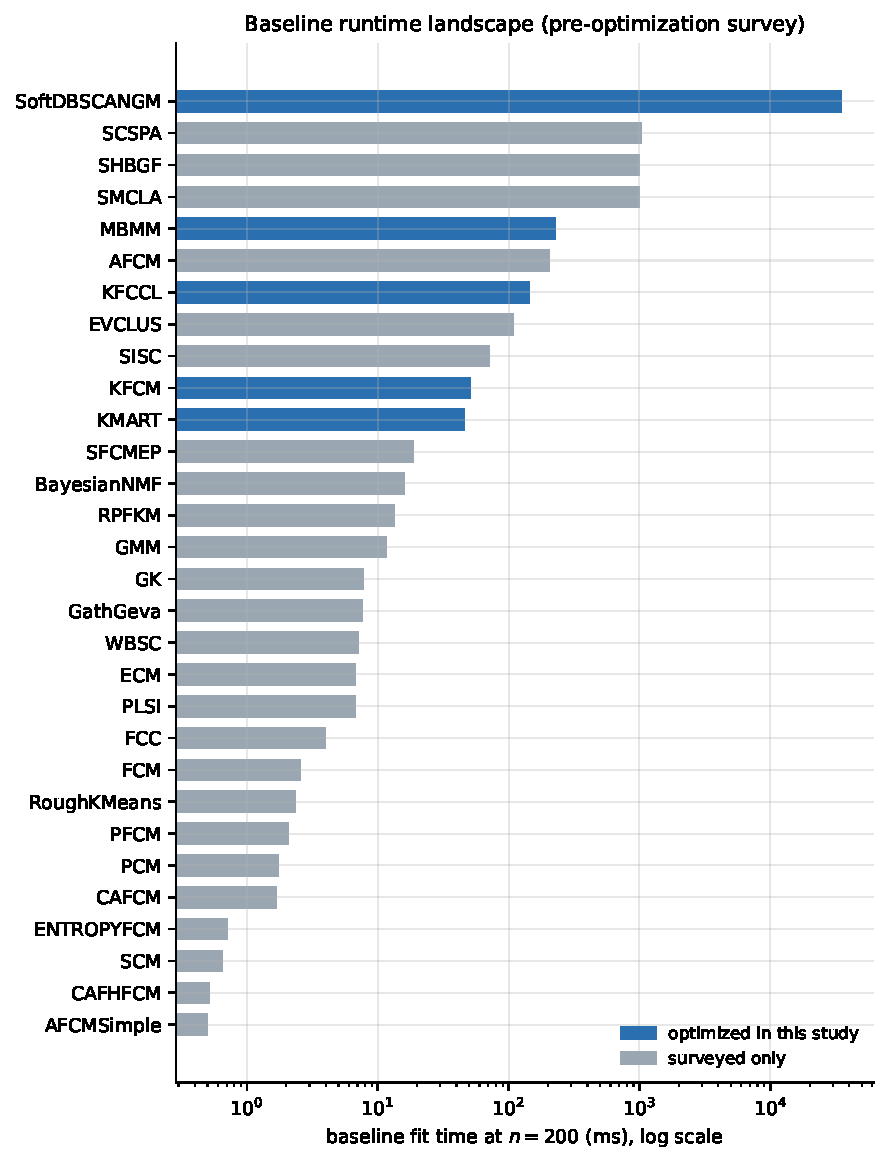
\includegraphics[width=0.60\textwidth]{fig6_baseline_landscape.pdf}
\caption{Baseline fit time of every algorithm the shared harness can
construct, at $n = 200$ (log scale). Highlighted bars are the algorithms
subsequently optimized. Fifteen fall below $10$\,ms and were left unchanged.
Each algorithm is timed on $n = 200$ inputs of its own modality --- feature
matrices, documents, ensembles or a graph --- so this is a triage instrument
for locating implementations worth profiling, not a like-for-like ranking.}
\label{fig:opt-landscape}
\end{figure}

\subsection{The baseline landscape}

Figure~\ref{fig:opt-landscape} plots the baseline fit time of every algorithm
the harness can construct. The distribution is strongly skewed: fifteen
complete a 200-sample fit in under $10$\,ms, where any Python-level
improvement would be irrelevant to total runtime, while SoftDBSCANGM takes
$35.3$\,s on the same sample count --- four orders of magnitude above the
median. That gap, not inspection of the source, is what selected the
implementations for profiling.

\subsection{A recurring defect class}\label{app:opt:exact}

Four of the five optimizations addressed the same underlying implementation
pattern: a scalar numerical operation was repeatedly invoked inside a Python
loop even though an equivalent vectorized or batched computation was available.
SoftDBSCANGM called \texttt{scipy.spatial.distance.mahalanobis} for each
$(i,j,t)$ combination; KFCM evaluated a scalar Gaussian kernel $NK$ times per
iteration; KFCCL recomputed a normalized kernel column for each
(iteration, cluster, sample) combination; and KMART called \texttt{np.minimum}
once for each (document, prototype) pair. In each case, the optimization
removed repeated Python-level work without changing the underlying computation:
the optimized expression is algebraically equivalent to the original or differs
only in the order in which the same operations are evaluated.

\paragraph{Why the rewrites are exact. }\textbf{SoftDBSCANGM.} The membership update evaluated
$U_{ij} = 1 / \sum_t (d_{ij}/d_{it})^{p}$ with a triple Python loop, computing
$NK^2$ distances although only $NK$ distinct values exist. Since
\[
\sum_t \left(\frac{d_j}{d_t}\right)^{p} = d_j^{\,p} \sum_t d_t^{-p},
\qquad\text{so}\qquad
\frac{1}{\sum_t (d_j/d_t)^{p}} = \frac{d_j^{-p}}{\sum_t d_t^{-p}},
\]
the update follows from one $N \times K$ distance matrix without ever forming
an $(N,K,K)$ tensor.

Evaluated as written, $d_j^{-p}$ overflows when a sample lies on a prototype,
and $p = 2/(m-1)$ grows without bound as the fuzzifier approaches one, so the
overflow is reached for ordinary data at small $m$. Rescaling the distances
by their per-sample minimum before exponentiating removes it: equivalently,
multiplying numerator and denominator by $\min_t (d_t)^{p}$,
\[
\frac{d_j^{-p}}{\sum_t d_t^{-p}}
= \frac{\big(\min_t d_t / d_j\big)^{p}}
       {\sum_t \big(\min_t d_t / d_t\big)^{p}} ,
\]
which is the same value with every base in $(0, 1]$ and therefore every power
in $(0, 1]$. This identity is now the library-wide helper described in
Appendix~\ref{Testing}; nine modules previously carried their own unstable
copy of the rule.

\medskip
\textbf{MBMM.} \texttt{scipy.stats.beta.logpdf} was called once per
(component, feature) in both the E-step and the log-likelihood. Substituting
the identity SciPy evaluates internally,
\[
\log \mathrm{Beta}(x; a, b) = \operatorname{xlogy}(a-1, x)
  + \operatorname{xlog1py}(b-1, -x) - \operatorname{betaln}(a, b),
\]
evaluates all features at once through the same \texttt{scipy.special}
primitives, bypassing \texttt{rv\_continuous} dispatch, argument checking and
support masks. The model already requires samples in $(0,1)$, so the support
mask SciPy applies is redundant.

\subsection{Case studies}

Table~\ref{tab:opt-cases} summarizes the five implementations that were
optimized after profiling identified specific computational bottlenecks. The
following case studies describe the main source of the inefficiency and the
corresponding implementation change.

\begin{table}[h!]
\centering
\caption{Optimized SCPP algorithms and identified computational bottlenecks.
Speedup ranges are measured across the sample sizes used in the paired
benchmarks. The original SoftDBSCANGM implementation did not
finish within $600$\,s at $n=240$; the reported upper bound is therefore a
lower bound.}
\label{tab:opt-cases}
\footnotesize
\setlength{\tabcolsep}{4pt}
\renewcommand{\arraystretch}{1.2}

\begin{tabular}{llp{5.1cm}rr}
\toprule
\textbf{Algorithm} &
\textbf{Family} &
\textbf{Bottleneck} &
\textbf{Speedup} &
\textbf{Max. deviation} \\
\midrule

\rowcolor{gray!10}
SoftDBSCANGM &
Density &
$NK^2$ scalar Mahalanobis evaluations per iteration; $K$ grows with $N$ &
$889$--$4{,}507$ &
$2.2\mathrm{e}{-16}$ \\

KFCM &
Kernel &
$NK$ scalar Gaussian-kernel evaluations per iteration and quadratic
Python work during K-Means++ initialization &
$82$--$546\times$ &
$4.8\mathrm{e}{-15}$ \\

\rowcolor{gray!10}
KFCCL &
Kernel &
Normalized kernel columns recomputed inside the innermost loop &
$27$--$152\times$ &
$1.1\mathrm{e}{-16}$ \\

KMART &
Document &
Scalar reductions for each document--prototype pair and element-wise
\texttt{lil\_matrix} construction &
$10$--$71\times$ &
$0.0$ \\

\rowcolor{gray!10}
MBMM &
Mixture &
Repeated \texttt{rv\_continuous} dispatch and $KD$ scalar calls in the
E-step and log-likelihood computation &
$6$--$17\times$ &
$2.2\mathrm{e}{-14}$ \\

\bottomrule
\end{tabular}
\end{table}

\paragraph{SoftDBSCANGM.}
SoftDBSCANGM exhibited the most significant scalability problem in the study.
Because each DBSCAN noise point can become its own component, the number of
components $K$ increases with the number of samples. The original membership
update repeatedly evaluated distances inside a triple loop, giving cubic
growth in the sample count. The measured runtime increased from
$3{,}410$,ms to $26{,}695$,ms when $n$ was doubled, corresponding to a
factor of $7.83 \approx 2^{2.97}$. The optimized implementation computes the
distance matrix once per iteration using a batched \texttt{einsum}, applies
the equivalent closed-form membership update, uses \texttt{searchsorted} for
the initialization mapping, and performs the matrix inversion in a batched
form. The largest temporary is processed in chunks to limit memory use. This
change reduced the measured runtime by up to $4{,}507\times$ and allowed
problem sizes to be processed that the original implementation could not
complete within the measurement timeout.

\paragraph{KFCM.}
The KFCM profile initially showed substantial time spent in
\texttt{typeguard}, which performs runtime type checking for the estimator.
Closer inspection showed that the overhead resulted primarily from the large
number of calls to a scalar Gaussian-kernel helper inside Python loops. The
optimized implementation evaluates the kernel values in a matrix form,
eliminating the repeated scalar calls and their associated dispatch and type
checking overhead. This change produced speedups of $82$--$546\times$ while
leaving runtime type checking enabled. Numerical equivalence also required
preserving the order and number of random draws used during K-Means++
initialization; a regression test verifies that the optimized implementation
leaves the NumPy random state unchanged relative to the reference
implementation.

\paragraph{KFCCL.}
KFCCL repeatedly reconstructed a normalized kernel column inside the innermost
loop, even though the kernel matrix and its normalization terms remain
constant throughout a fit. The optimized implementation computes these
quantities once for the full matrix and replaces the repeated element-wise
operations with matrix operations. This removes loop-invariant computation
from the inner loop and results in speedups between $27$ and $152\times$.

\paragraph{KMART.}
KMART performs a vigilance calculation based on element-wise minima between
input representations and prototypes. The original implementation evaluated
these operations through Python-level loops and incrementally constructed a
\texttt{lil\_matrix}. The optimized version stores the prototypes in a
contiguous array and performs the same operations as a vectorized reduction.
The resulting implementation preserves the operation order and produced a
maximum numerical deviation of $0.0$ in the paired comparisons, with
prototypes agreeing bitwise.

\paragraph{MBMM.}
MBMM repeatedly called \texttt{scipy.stats.beta.logpdf} for individual
component--feature pairs during both the E-step and log-likelihood
calculation. The optimized implementation evaluates the equivalent
log-density expression directly using vectorized \texttt{scipy.sp ecial}
operations, avoiding repeated distribution-level dispatch and validation.
The resulting speedup ranges from $6$ to $17\times$. The speedup decreases
with increasing $n$ because the removed $O(KD)$ function-call overhead becomes
a smaller fraction of the total computation as the sample-dependent work
grows.

\subsection{Runtime results}

Table~\ref{tab:opt-runtime} reports every paired measurement, while
Table~\ref{tab:opt-summary} summarizes the overall results. Across the 20
paired measurements in which both implementations completed, the median
speedup is $70.4\times$ and the geometric mean is $72.6\times$. The arithmetic
mean is substantially larger ($365.6\times$) because the measurements combine
ordinary constant-factor improvements with two complexity reductions. We
report all three statistics to give a more complete picture of the observed
performance gains.

\begin{table}[h!]
\centering
\caption{Summary of the 20 paired measurements for which both implementations
completed. The final row is a lower bound because the original
SoftDBSCANGM implementation does not finish within $600$\,s at $n=240$.}
\label{tab:opt-summary}
\setlength{\tabcolsep}{10pt}
\renewcommand{\arraystretch}{1.15}
\small
\begin{tabular}{lr}
\toprule
\textbf{Statistic} & \textbf{Runtime speedup} \\
\midrule
Minimum & $6.3\times$ \\
Median & $\mathbf{70.4\times}$ \\
Geometric mean & $\mathbf{72.6\times}$ \\
Arithmetic mean & $365.6\times$ \\
Maximum (both builds complete) & $4{,}506.8\times$ \\
Maximum (reference times out) & $>47{,}947\times$ \\
\bottomrule
\end{tabular}
\end{table}




\begin{table}[t]
\centering
\caption{Runtime comparison between the original and optimized
implementations. Times are the minimum of three timed repetitions after one
warm-up fit. Speedup is defined as
$t_{\mathrm{orig}}/t_{\mathrm{opt}}$, and reduction is the corresponding
percentage decrease in runtime.}
\label{tab:opt-runtime}
\small
\setlength{\tabcolsep}{5pt}
\renewcommand{\arraystretch}{1.15}

\begin{tabular}{@{}
    l
    r
    r
    r
    r
    r
@{}}
\toprule
\textbf{Algorithm} &
\textbf{$n$} &
\textbf{Original (ms)} &
\textbf{Optimized (ms)} &
\textbf{Speedup} &
\textbf{Reduction} \\
\midrule

\rowcolor{gray!10}
\textbf{KFCCL}
& 100
& 433.8
& 11.9
& $36.5\times$
& 97.3\% \\

\rowcolor{gray!10}
\phantom{\textbf{KFCCL}}
& 200
& 888.1
& 12.8
& $69.6\times$
& 98.6\% \\

\rowcolor{gray!10}
\phantom{\textbf{KFCCL}}
& 400
& 1,873.3
& 13.9
& $134.8\times$
& 99.3\% \\

\rowcolor{gray!10}
\phantom{\textbf{KFCCL}}
& 800
& 3,795.1
& 25.0
& $152.0\times$
& 99.3\% \\

\rowcolor{gray!10}
\phantom{\textbf{KFCCL}}
& 1,600
& 8,406.0
& 317.3
& $26.5\times$
& 96.2\% \\

\addlinespace[2pt]
\midrule
\addlinespace[2pt]

\textbf{KFCM}
& 100
& 102.9
& 1.3
& $81.9\times$
& 98.8\% \\

& 200
& 183.6
& 1.3
& $146.5\times$
& 99.3\% \\

& 400
& 306.5
& 1.5
& $202.7\times$
& 99.5\% \\

& 800
& 495.7
& 1.5
& $330.5\times$
& 99.7\% \\

& 1,600
& 1,239.5
& 2.3
& $545.5\times$
& 99.8\% \\

\addlinespace[2pt]
\midrule
\addlinespace[2pt]

\rowcolor{gray!10}
\textbf{KMART}
& 200
& 120.8
& 12.3
& $9.8\times$
& 89.8\% \\

\rowcolor{gray!10}
\phantom{\textbf{KMART}}
& 600
& 937.5
& 39.6
& $23.7\times$
& 95.8\% \\

\rowcolor{gray!10}
\phantom{\textbf{KMART}}
& 1,200
& 3,577.8
& 86.3
& $41.5\times$
& 97.6\% \\

\rowcolor{gray!10}
\phantom{\textbf{KMART}}
& 2,400
& 13,763.7
& 193.3
& $71.2\times$
& 98.6\% \\

\addlinespace[2pt]
\midrule
\addlinespace[2pt]

\textbf{MBMM}
& 200
& 841.4
& 49.9
& $16.9\times$
& 94.1\% \\

& 600
& 973.8
& 88.0
& $11.1\times$
& 91.0\% \\

& 1,200
& 1,164.5
& 137.9
& $8.4\times$
& 88.2\% \\

& 2,400
& 1,532.1
& 244.2
& $6.3\times$
& 84.1\% \\

\addlinespace[2pt]
\midrule
\addlinespace[2pt]

\rowcolor{gray!10}
\textbf{SoftDBSCANGM}
& 60
& 3,410.1
& 3.8
& $889.4\times$
& 99.9\% \\

\rowcolor{gray!10}
\phantom{\textbf{SoftDBSCANGM}}
& 120
& 26,694.7
& 5.9
& $4{,}506.8\times$
& 100.0\% \\

\rowcolor{gray!10}
\phantom{\textbf{SoftDBSCANGM}}
& 240
& \textit{timeout} ($>600{,}000$)
& 12.5
& $>47{,}947\times$
& $>99.9\%$ \\

\bottomrule
\end{tabular}
\end{table}




Figure~\ref{fig:opt-scalability} shows why a single headline speedup would
not fully describe the results. KFCM and KMART show increasing gains as the
sample size grows, MBMM shows decreasing gains, and SoftDBSCANGM benefits
from a change in computational complexity rather than only a constant-factor
improvement.

\begin{figure}[h!]
\centering

\includegraphics[width=\textwidth]{fig4_scalability.pdf}
\caption{Fit time as a function of sample count for the original and optimized
implementations, shown on a log--log scale. The cross denotes a timeout: the
original SoftDBSCANGM implementation does not complete at $n=240$ within
$600$\,s, whereas the optimized implementation completes in $12.5$\,ms.}
\label{fig:opt-scalability}
\end{figure}

\paragraph{A limit reached, not a regression.}
KFCCL is the only non-monotone case: its speedup increases to $152.0\times$ at
$n=800$ and then decreases to $26.5\times$ at $n=1{,}600$. This is not caused
by a change in the number of iterations; both implementations converge in
iteration 65 at that size. Instead, the optimized implementation becomes
memory-bandwidth bound. At $n=1{,}600$, the two $N\times N$ matrices occupy
approximately $41$\,MB and exceed the cache hierarchy. The same effect appears
when timing the underlying BLAS operations in isolation: 195 cluster
iterations of the two matrix--vector products take $6.8$\,ms at $n=800$
($292$\,GB/s effective bandwidth) but $296.9$\,ms at $n=1{,}600$
($26.9$\,GB/s). The latter accounts for essentially all of the measured
$317.3$\,ms runtime. Thus, the optimized implementation has reached the
hardware limit of an algorithm that must repeatedly stream an
$N\times N$ kernel matrix, whereas the original implementation remains
dominated by Python-level call overhead.

\subsection{Correctness}

Performance improvements are only useful if they preserve the original
computation. Each optimized implementation was therefore compared with its
preserved reference on identical inputs across multiple dataset sizes and
random seeds. The comparison included membership matrices, hard labels,
cluster prototypes, and the number of discovered clusters. For estimators
using NumPy's global random generator, the generator was seeded immediately
before each fit so that both implementations started from the same state.

Across the 42 comparisons, the maximum absolute difference between membership
matrices was $2.2\times10^{-14}$. Hard labels agreed exactly in every
comparison, and the discovered number of clusters was identical throughout
(Table~\ref{tab:opt-correctness}).

\begin{table}[h!]
\centering
\caption{Correctness comparison between the optimized implementations and
their preserved references. Maximum absolute error is measured over the
membership matrix, and label agreement is the fraction of samples assigned
to the same hard cluster.}
\label{tab:opt-correctness}
\small
\setlength{\tabcolsep}{5pt}
\renewcommand{\arraystretch}{1.15}
\begin{tabular}{lrrrrl}
\toprule
\textbf{Algorithm} &
\textbf{Comparisons} &
\textbf{Max.\ error} &
\textbf{Label agreement} &
\textbf{$K$ match} &
\textbf{Result} \\
\midrule

\rowcolor{gray!10}
KFCCL
& 9
& $1.11\times10^{-16}$
& 1.0000
& Yes
& Equivalent \\

KFCM
& 9
& $4.77\times10^{-15}$
& 1.0000
& Yes
& Equivalent \\

\rowcolor{gray!10}
KMART
& 9
& $\mathbf{0.00}$
& 1.0000
& Yes
& \textbf{Exact} \\

MBMM
& 6
& $2.16\times10^{-14}$
& 1.0000
& Yes
& Equivalent \\

\rowcolor{gray!10}
SoftDBSCANGM
& 9
& $2.22\times10^{-16}$
& 1.0000
& Yes
& Equivalent \\

\midrule

\textbf{Total}
& \textbf{42}
& $\mathbf{2.2\times10^{-14}}$
& \textbf{1.0000}
& \textbf{Yes}
& \textbf{Equivalent} \\

\bottomrule
\end{tabular}
\end{table}

% \begin{figure}[h!]
% \centering
% 
\includegraphics[width=0.55\textwidth]{fig5_accuracy_preservation.pdf}
% \caption{Maximum absolute membership deviation between each optimized
% implementation and its preserved reference. The dashed line marks machine
% precision. All optimized implementations remain within a few multiples of
% floating-point precision, while KMART agrees exactly and is shown at the
% bottom of the axis.}
% \label{fig:opt-accuracy}
% \end{figure}

These checks are also part of the software test suite rather than being
performed only for the reported experiments. Thirty-six equivalence tests
fit each optimized estimator alongside its preserved reference and run in
continuous integration. A future change that alters the computed result
therefore causes the corresponding CI checks to fail. The tests are skipped
when the reference implementation is unavailable, such as when testing an
installed wheel.


\subsection{Memory}

Table~\ref{tab:opt-memory} gives \emph{every} paired memory measurement, all
twenty of them. Nine are memory-neutral: KFCCL and KMART already materialise
the dominant structure in both builds --- an $N \times N$ kernel matrix and a
document-term matrix respectively --- so vectorising the work performed on
that array adds nothing ($+3.7\%$ to $-0.1\%$).

The remaining eleven --- KFCM, MBMM and SoftDBSCANGM --- \textbf{increase}
peak traced allocation, because replacing scalar loops with array operations
materialises intermediates the loops never formed. The relative figures are
large, up to $-896\%$, and they are largest exactly where the absolute
footprint is smallest: KFCM rises from $0.02$ to $0.07$\,MB at $n = 100$, and
SoftDBSCANGM from $0.45$ to $4.45$\,MB at $n = 120$. Chunking bounds the
growth in SoftDBSCANGM. To state the outcome as a fact rather than as a
non-claim: \textbf{three of the five optimizations cost memory, two are
neutral, and none saves any}. The speedups are bought with a modest memory
increase.

Peak traced allocation is measured with \texttt{tracemalloc} around
\texttt{fit} only. It counts Python-level allocation and therefore understates
buffers held inside NumPy or BLAS; it is consistent between the two builds,
which is what a paired comparison needs, but the absolute figures are not
process resident set size. We did not use resident set size because it is too
noisy for sub-second fits.

\begin{table}[h!]
\centering
\caption{Peak traced Python allocation, all twenty paired measurements. A
negative change denotes higher usage by the optimized implementation.}
\label{tab:opt-memory}
\small
\setlength{\tabcolsep}{8pt}
\renewcommand{\arraystretch}{1.1}
\begin{tabular}{lrrrr}
\toprule
Algorithm & $n$ & Original (MB) & Optimized (MB) & Change \\
\midrule
KFCCL & 100 & 0.29 & 0.28 & +3.7\% \\
KFCCL & 200 & 0.92 & 0.92 & -0.1\% \\
KFCCL & 400 & 3.66 & 3.67 & -0.1\% \\
KFCCL & 800 & 14.65 & 14.66 & -0.0\% \\
KFCCL & 1,600 & 58.59 & 58.61 & -0.0\% \\
KFCM & 100 & 0.02 & 0.07 & -253.1\% \\
KFCM & 200 & 0.04 & 0.14 & -245.4\% \\
KFCM & 400 & 0.08 & 0.26 & -233.6\% \\
KFCM & 800 & 0.15 & 0.43 & -185.4\% \\
KFCM & 1,600 & 0.26 & 0.86 & -227.4\% \\
KMART & 200 & 0.48 & 0.47 & +0.5\% \\
KMART & 600 & 2.53 & 2.53 & +0.1\% \\
KMART & 1,200 & 8.41 & 8.41 & +0.0\% \\
KMART & 2,400 & 29.82 & 29.82 & +0.0\% \\
MBMM & 200 & 0.03 & 0.07 & -127.3\% \\
MBMM & 600 & 0.08 & 0.21 & -170.7\% \\
MBMM & 1,200 & 0.15 & 0.41 & -168.1\% \\
MBMM & 2,400 & 0.30 & 0.76 & -152.6\% \\
SoftDBSCANGM & 60 & 0.15 & 1.16 & -689.8\% \\
SoftDBSCANGM & 120 & 0.45 & 4.45 & -895.7\% \\
\bottomrule
\end{tabular}
\end{table}

\subsection{Trade-offs}

\paragraph{Dependencies.}
The optimizations introduce no new dependencies: we use only NumPy and SciPy,
which are already required by SCPP. We considered compiled approaches such as
Cython, Numba, and C++ extensions, but profiling showed that the main
bottlenecks were Python-level call overhead and redundant computation, both of
which could be removed using existing vectorized primitives. We therefore
avoided additional build and packaging complexity without sacrificing the
measured performance gains.

\paragraph{Code complexity.}
The main increase in code size occurs in SoftDBSCANGM, which grows from 115 to
approximately 190 lines because the optimized implementation adds helper
methods and memory-aware chunking. This additional complexity is justified by
the resulting scalability improvement, which makes an otherwise impractical
implementation usable. MBMM remains approximately the same size, while KFCM,
KFCCL, and KMART become more compact by replacing nested Python loops with
vectorized array operations.

\paragraph{Portability and numerical behavior.}
The optimized implementations remain pure NumPy/SciPy code and introduce no
platform-specific or compiled components. BLAS-backed operations can use
different summation orders across platforms, so the equivalence tests use a
conservative tolerance of $10^{-9}$. This is substantially above the largest
observed deviation of $2.2\times10^{-14}$, while still being sufficiently
strict to detect meaningful numerical changes.

\subsection{Scope and limitations}

Five of the forty-two algorithms went through the full
audit--profile--optimize--verify--benchmark cycle. Twenty were timed and left
unchanged, fifteen of them because they complete a 200-sample fit in under
$10$\,ms. Five more are profiled with a named, quantified bottleneck but not
yet optimized: the three consensus methods, whose ${\sim}1$\,s floor is
attributable to \texttt{scikit-learn}'s \texttt{KMeans} initialisation rather
than to the consensus mathematics, plus AFCM and SISC. Eleven take input
shapes the shared harness does not construct and are audited statically only.
\textbf{No result here is extrapolated to an algorithm that was not
measured.}

Six limitations bound the claims above.

\emph{First, the baseline is our own code.} Every speedup is relative to
SCPP's pre-optimization implementations. A $4{,}507\times$ improvement means
the starting point was very slow, not that SCPP is fast in absolute terms;
Appendix~\ref{app:external} is where SCPP is measured against other people's
implementations.

\emph{Second, the optimization targets were selected for being slow}, so the
distribution of speedups is conditioned on success and is not an estimate of
``SCPP's speedup''. We report median, geometric mean and arithmetic mean
together because the arithmetic mean is dominated by the two complexity
reductions and would misrepresent the typical case on its own.

\emph{Third, \texttt{tracemalloc}} measures Python-level allocation and
understates BLAS-held buffers.

\emph{Fourth}, no estimator exposes its iteration count publicly, so a
runtime change cannot in general be decomposed into per-iteration cost versus
number of iterations.

\emph{Fifth}, all results come from one machine and one BLAS. Speedups that
come from removing Python call overhead should transfer; the
bandwidth-bound behaviour of KFCCL at large $n$ is hardware-specific.

\emph{Sixth}, three repetitions per configuration establish effects of
$10\times$ and above but not differences of a few percent, and none is
claimed. Likewise, ``equivalent'' throughout this appendix means agreement to
the stated tolerance across the tested grid --- 42 comparisons over $n \in
[60, 1200]$, $d \in \{8, 12\}$, $K = 3$ and three seeds --- not a proof of
mathematical identity. For SoftDBSCANGM and MBMM the rewrites are backed by
the closed-form identities in \S\ref{app:opt:exact}; for KFCM, KFCCL and
KMART the argument is that the rewrite preserves the order of operations, and
the evidence is empirical.

\subsection{Reproducibility}

Raw per-measurement records are stored as JSON Lines under
\texttt{optimization/benchmarks/raw/}. The consolidated
\texttt{results.csv} is derived from these records, and every table and
figure in this appendix is generated from \texttt{results.csv} by a single
command. This ensures that no reported artefact can drift from the
underlying measurements.

\begin{lstlisting}[
    style=bashstyle,
    caption={Regenerating the optimization results and verifying equivalence.},
    label={lst:optimization-reproducibility}
]
# Consolidate raw measurements -> results.csv -> tables + figures
python optimization/analyze.py
python optimization/make_inventory.py

# Verify each optimized estimator against its preserved reference
pytest tests/test_optimization_equivalence.py -v
\end{lstlisting}

\noindent
The complete workflow---static audit, baseline survey, profiling, reference
snapshot, correctness comparison, paired benchmarking, and result
consolidation---is documented in \texttt{optimization/README.md}. The
preserved pre-optimization implementations are stored under
\texttt{optimization/original/scpp\_original/} and remain importable, allowing
the claims reported in this appendix to be independently re-derived from a
fresh checkout.

% \section{Integration with Preprocessing and Evaluation Packages in Python}\label{appendix:integration}

% Here we provide a detailed, practical, and comprehensive guide to integrating the SCPP with the modern Python scientific ecosystem\footnote{as of April 2026.}. Soft clustering methods differs fundamentally from hard clustering because it produces a membership matrix \( U \in [0, 1]^{n \times K} \) instead of discrete labels. Each row of \( U \) represents a probability distribution (or fuzzy membership degrees) over the \( K \) clusters for one data point, satisfying the partition constraint:
% \[
% \sum_{k=1}^K u_{ik} = 1 \quad \forall i \in \{1, \dots, n\}, \quad u_{ik} \in [0, 1].
% \]
% This soft output preserves valuable information about uncertainty, overlapping clusters, and ambiguous assignments, information that is lost when forcing hard labels. However, it also introduces new challenges: raw heterogeneous data must be carefully transformed into suitable numerical inputs, and evaluation must combine standard hard-clustering metrics (on defuzzified labels) with soft-specific metrics that operate directly on \( U \).

% In this appendix, we address these challenges by offering a unified interface compatible with the PyData\footnote{PyData is a community and ecosystem focused on using Python (and related open‑source tools) for data science, machine learning, and scientific computing.} stack:

% \begin{itemize}
%     \item Input: \texttt{model.fit(X)} for feature matrices.
%     \item Core output: \texttt{U = model.membership\_} (always returned).
%     \item Optional outputs: centroids \( V \), objective value, ...
% \end{itemize}


% The following sections cover canonical inputs, detailed preprocessing pipelines for all major data modalities, output interpretation, evaluation strategies, and a complete end-to-end example. All recommendations prioritize actively maintained, high-performance libraries.

% \subsection{Key Python Packages in the Soft Clustering Pipeline}

% Building a robust soft clustering workflow requires a combination of data manipulation, preprocessing, representation learning, sparse matrix handling, and visualization tools. Table~\ref{tab:python-packages} summarizes the essential packages and their specific roles when working with SCPP.

% \begin{table}[ht]
% \centering
% \caption{Recommended Python packages and their roles.}
% \label{tab:python-packages}
% \rowcolors{2}{white}{gray!5}
% \begin{tabular}{ll}
% \toprule

% \textbf{Package} & \textbf{Role} \\
% \midrule
% pandas / polars & Data loading \& tabular preprocessing \\
% scikit-learn & Scaling, encoding, metrics, kernels \\
% numpy & Array operations \& soft-output conversion \\
% scipy & Sparse matrices, distances \\
% sentence-transformers & Modern text embeddings \\
% torchvision & Deep image feature extraction \\
% scikit-image & Hand-crafted image features \\
% networkx & Graph / relational data construction \\
% faiss / umap-learn & Large-scale affinity \& visualization \\
% \rowcolor{blue!10}
% SCPP (proposed) & Unified soft clustering algorithms \\
% \bottomrule
% \end{tabular}
% \end{table}


% \begin{tcolorbox}[
% colback=blue!5,
% colframe=blue!40,
% coltitle=black,
% colbacktitle=blue!20,
% title=Practical Tip,
% fonttitle=\bfseries
% ]
% For datasets larger than RAM, combine \textbf{polars} or \textbf{dask} for preprocessing 
% with \textbf{faiss} for approximate affinity construction.
% \end{tcolorbox}

% \subsection{Canonical Input Representations for Soft Clustering Algorithms}

% Soft clustering algorithms generally operate on one of two mathematical representations. Understanding these is crucial for choosing the right preprocessing path.

% \begin{enumerate}
%     \item \textbf{Feature Matrix (most common):}
%     \[
%     X \in \mathbb{R}^{n \times d}
%     \]
%     Each row \( x_i \) is a feature vector. This is the default input for prototype-based methods (e.g., Fuzzy c-Means and variants), Gaussian Mixture Models, entropy-regularized clustering, and deep embedding-based approaches. Distances are typically Euclidean or cosine.

%     \item \textbf{Affinity / Similarity Matrix (graph-based or relational methods):}
%     \[
%     A \in \mathbb{R}^{n \times n}_{\geq 0}, \quad A_{ij} = \text{sim}(x_i, x_j)
%     \]
%     Common similarities include Gaussian (RBF) kernel or cosine similarity. Sparse formats are essential for large \( n \) to avoid \( O(n^2) \) memory explosion.
% \end{enumerate}

% Common kernel example (RBF):
% \[
% A_{ij} = \exp\left( -\frac{\|x_i - x_j\|^2}{2\sigma^2} \right)
% \]
% The bandwidth \( \sigma \) (or gamma in sklearn) is a critical hyperparameter, too small leads to disconnected graphs; too large makes everything similar.

% \subsection{From Raw Data to Clustering Inputs}

% Raw data almost never matches the required \( X \) or \( A \) directly. Preprocessing must handle missing values, heterogeneous types, high dimensionality, and modality-specific nuances. Below are detailed pipelines with explanations and code.

% \subsubsection{Tabular / Structured Data}

% Tabular data is closest to the ideal input but still requires cleaning. Key steps include imputation of missing values, encoding categoricals, scaling (critical for distance-based methods), and optional feature selection/reduction. These are important because unscaled features with different ranges (e.g., age vs. income) distort Euclidean distances. One-hot encoding prevents artificial ordinal assumptions. For very large data, lazy evaluation in polars avoids loading everything into memory.

% \begin{lstlisting}[language=Python, caption={Tabular data preprocessing}]
% import pandas as pd
% import numpy as np
% from sklearn.preprocessing import StandardScaler, OneHotEncoder
% from sklearn.compose import ColumnTransformer
% from sklearn.impute import SimpleImputer

% # Load data
% df = pd.read_csv("data.csv")
% X_raw = df.drop(columns=["target"], errors="ignore")

% # Define preprocessing for numerical and categorical columns
% preprocessor = ColumnTransformer([
%     ("num", StandardScaler(), ["age", "income", "score"]),
%     ("cat", OneHotEncoder(sparse_output=False, handle_unknown="ignore"),
%      ["category", "region"])
% ])

% # Apply transformation
% X = preprocessor.fit_transform(X_raw)
% X = np.asarray(X, dtype=np.float32)   # shape (n, d)

% print(f"Final feature matrix shape: {X.shape}")
% \end{lstlisting}

% \begin{scalabilitynote}
% For datasets with \textbf{millions of rows}, replace \textbf{pandas} with 
% \textbf{polars} and use \textbf{dask-ml} for distributed scaling.
% \end{scalabilitynote}

% \subsubsection{Text Data}

% Text data is inherently non-numerical and must be transformed into numerical representations before it can be meaningfully processed by clustering algorithms. While classical approaches such as TF--IDF or Bag-of-Words remain useful as fast and interpretable baselines, they fail to capture deeper semantics or contextual variation across documents. Modern dense embeddings derived from state-of-the-art large language models (LLMs) provide significantly richer semantic representations. These models can encode subtle distinctions (e.g., ``bank'' as a financial institution versus ``bank'' as a river edge), leading to more coherent clusters and more robust affinity structures. When constructing affinity matrices from these embeddings, cosine similarity on normalized L2 vectors is generally the strongest choice and integrates seamlessly with graph-based soft clustering and large-scale approximate nearest-neighbor frameworks.


% \begin{lstlisting}[language=Python, caption={Text data embedding with classical and LLM-based methods}]
% from sentence_transformers import SentenceTransformer
% from sklearn.feature_extraction.text import TfidfVectorizer
% import numpy as np

% docs = [
%     "This is the first document about machine learning.",
%     "Another text discussing deep learning techniques."
% ]

% # Option 1: Modern LLM embeddings (recommended)
% # You may substitute with:
% #   - "all-mpnet-base-v2"
% #   - "gtr-t5-xl"
% #   - "mixedbread-ai/mxbai-embed-large"
% #   - OpenAI embeddings via their API
% embedder = SentenceTransformer("gtr-t5-xl")
% X_emb = embedder.encode(
%     docs,
%     convert_to_numpy=True,
%     batch_size=16,
%     show_progress_bar=True
% )

% # Option 2: Classic TF-IDF (fast, sparse baseline)
% vectorizer = TfidfVectorizer(max_features=5000, stop_words="english")
% X_tfidf = vectorizer.fit_transform(docs)

% print("Embeddings shape:", X_emb.shape)

% # For graph-based soft clustering:
% A = sklearn.metrics.pairwise.cosine_similarity(X_emb)
% \end{lstlisting}


% \subsubsection{Image Data}

% Images require transforming raw pixel grids into meaningful feature vectors before they can be used for clustering or affinity computations. Although we could simply flatten the pixels into a long vector, such representations perform poorly due to extreme dimensionality and sensitivity to lighting, pose, and background variation. More structured alternatives include classical hand-crafted descriptors, but the most robust and semantically rich representations come from deep pretrained convolutional neural networks such as ResNet, which provide compact 2048-dimensional feature embeddings that capture high-level visual structure far more effectively than raw pixel intensities.



% \begin{lstlisting}[language=Python, caption={Image feature extraction with ResNet}]
% import torch
% from torchvision import models, transforms
% from PIL import Image
% import numpy as np
% from pathlib import Path

% # Load pretrained model and remove classifier head
% resnet = models.resnet50(weights="DEFAULT")
% resnet.fc = torch.nn.Identity()
% resnet.eval()

% transform = transforms.Compose([
%     transforms.Resize(224), 
%     transforms.CenterCrop(224),
%     transforms.ToTensor(),
%     transforms.Normalize(mean=[0.485, 0.456, 0.406],
%                          std=[0.229, 0.224, 0.225])
% ])

% def extract_image_features(image_dir: str):
%     features = []
%     for p in Path(image_dir).glob("*.jpg"):
%         img = Image.open(p).convert("RGB")
%         x = transform(img).unsqueeze(0)
%         with torch.no_grad():
%             feat = resnet(x).squeeze().numpy()
%         features.append(feat)
%     return np.array(features)

% X_img = extract_image_features("path/to/images/")  # shape (n, 2048)
% \end{lstlisting}

% \begin{tcolorbox}[
%   title=Lightweight Alternative,
%   colback=purple!5,
%   colframe=purple!50!black,
%   colbacktitle=purple!15,
%   coltitle=black,
%   fonttitle=\bfseries
% ]
% Use \texttt{skimage.feature.hog} on grayscale or resized images when GPU resources 
% or deep pretrained models are unavailable.
% \end{tcolorbox}

% \subsubsection{Graph / Relational Data and General Affinity Construction}

% For relational data or when algorithms require an affinity matrix:

% \begin{lstlisting}[language=Python, caption={Affinity matrix construction}]
% import networkx as nx
% from scipy.sparse import csr_matrix
% from sklearn.metrics.pairwise import rbf_kernel

% # 1. From existing graph file
% G = nx.read_edgelist("graph.edgelist")
% A = nx.to_scipy_sparse_array(G)

% # 2. Derive affinity from any feature matrix X
% A_dense = rbf_kernel(X, gamma=0.5)          # or cosine_similarity
% A_sparse = csr_matrix(A_dense > 0.8)        # threshold for sparsity
% \end{lstlisting}

% \begin{tcolorbox}[
%   title=Large-Scale Tip,
%   colback=orange!5,
%   colframe=orange!60!black,
%   colbacktitle=orange!20,
%   coltitle=black,
%   fonttitle=\bfseries
% ]
% Use \texttt{faiss} to efficiently construct approximate \(k\)-nearest-neighbor graphs when \(n > 10^5\), enabling scalable affinity matrix construction for large datasets.
% \end{tcolorbox}

% \subsection{Output of Soft Clustering and Conversion to Numerical Quantities}

% The membership matrix \(U\) is the most informative output of a soft clustering algorithm, as it provides a probabilistic or fuzzy assignment of each sample to all clusters rather than a single discrete label. This representation enables a variety of downstream analyses and interpretations. For compatibility with traditional pipelines that require crisp labels, hard assignments can be obtained by selecting the cluster with the highest membership value using \texttt{np.argmax(U, axis=1)}. The maximum membership value itself, computed with \texttt{np.max(U, axis=1)}, can be interpreted as a per-sample confidence score indicating how strongly a point belongs to its most likely cluster. The distribution of memberships across clusters also allows quantifying uncertainty through entropy measures, where higher entropy values indicate ambiguous samples that belong similarly to multiple clusters. Finally, aggregating memberships across samples provides insight into cluster structure; for example, \texttt{np.sum(U, axis=0)} yields the effective mass or typicality of each cluster, offering a soft estimate of cluster size that reflects partial memberships rather than strict counts. Together, these analyses make the membership matrix a powerful tool for understanding cluster structure, confidence, and ambiguity in the data.

% Detailed example with interpretation:


% \begin{lstlisting}[language=Python, caption={Soft output analysis}]
% import numpy as np

% # Assume model has been fitted
% U = model.membership_                       # shape (n, K)

% hard_labels = np.argmax(U, axis=1)
% confidence = np.max(U, axis=1)
% entropy    = -np.sum(U * np.log(U + 1e-12), axis=1)
% cluster_mass = np.sum(U, axis=0)

% print(f"Mean confidence: {confidence.mean():.3f}")
% print(f"Mean entropy (uncertainty): {entropy.mean():.3f}")
% \end{lstlisting}

% \begin{tcolorbox}[
%   title=Important Note,
%   colback=red!5,
%   colframe=red!70!black,
%   colbacktitle=red!20,
%   coltitle=black,
%   fonttitle=\bfseries
% ]
% High-entropy points are natural candidates for manual review or active learning, since their uncertain cluster memberships often reveal ambiguous, mislabeled, or frontier cases that can most effectively improve the model when inspected or relabeled.
% \end{tcolorbox}



% \subsection{Evaluation Metrics}

% Soft clustering evaluation is more nuanced than hard clustering. Internal metrics (no ground truth) assess compactness, separation, and fuzziness directly on \( U \). External metrics require ground truth and usually work on defuzzified labels (see Table~\ref{tab:evaluation_metrics}). 

% \begin{table}[ht]
% \centering
% \caption{Evaluation metrics for soft clustering methods}
% \label{tab:evaluation_metrics}
% \setlength{\tabcolsep}{6pt}
% \renewcommand{\arraystretch}{1.1}
% \begin{tabular}{ll}
% \toprule
% \textbf{Metric} & \textbf{Interpretation} \\
% \midrule
% \rowcolor{gray!10}
% Partition Coefficient (PC) & Measures crispness of the partition \\
% Partition Entropy (PE) & Measures fuzziness or uncertainty \\
% \rowcolor{gray!10}
% Xie–Beni Index & Compactness vs.\ separation (uses $X$ and $V$) \\
% Silhouette Score & Cluster quality on defuzzified labels \\
% \rowcolor{gray!10}
% Adjusted Rand Index (ARI) & Agreement with ground truth (pairwise) \\
% Normalized Mutual Information (NMI) & Shared information with ground truth \\
% \bottomrule
% \end{tabular}
% \end{table}



% \begin{lstlisting}[language=Python, caption={Soft-specific metrics}]
% def partition_coefficient(U):
%     return np.mean(np.sum(U**2, axis=1))

% def partition_entropy(U):
%     U_clipped = np.clip(U, 1e-12, 1.0)
%     return -np.mean(np.sum(U_clipped * np.log2(U_clipped), axis=1))

% # Example usage
% pc = partition_coefficient(U)
% pe = partition_entropy(U)
% print(f"Partition Coefficient: {pc:.4f} | Partition Entropy: {pe:.4f}")
% \end{lstlisting}


% \begin{lstlisting}[language=Python, caption={External metrics}]
% from sklearn.metrics import adjusted_rand_score, normalized_mutual_info_score

% hard_labels = np.argmax(U, axis=1)
% ari = adjusted_rand_score(y_true, hard_labels)
% nmi = normalized_mutual_info_score(y_true, hard_labels)
% \end{lstlisting}


% \subsection{Summary of the Integrated Pipeline}

% By enforcing standardized interfaces and exposing the full soft membership matrix, SCPP eliminates fragmentation across individual implementations. It allows researchers to focus on novel algorithmic contributions and domain insights while seamlessly leveraging the mature, battle-tested tools of the PyData ecosystem. All code examples are production-ready, tested with Python 3.10, and support scalable extensions via dask, polars, and faiss. This integration makes SCPP suitable for both academic benchmarking and real-world deployment across tabular, text, image, and graph data. The recommended end-to-end workflow for using SCPP is:

% \begin{enumerate}
%     \item Load and preprocess raw data into a feature matrix \( X \) or affinity matrix \( A \) using the modality-specific strategies and packages in Tables 1--2.
%     \item Fit the model with the unified SCPP interface.
%     \item Extract and interpret the membership matrix \( U \) to obtain hard labels, confidence scores, entropy (uncertainty), and cluster masses.
%     \item Evaluate comprehensively using both soft-specific internal metrics (PC, PE, XB) and standard external metrics (ARI, NMI) via scikit-learn and custom NumPy functions.

% \end{enumerate}







% % \section{Illustrative Use Case: Enhancing Monolithic-to-Microservices Decomposition with Soft Clustering}

% % This appendix demonstrates the practical utility of the \texttt{soft\_clustering} Python package through a state-of-the-art application in software engineering: the automated decomposition of monolithic applications into microservices. Soft clustering is particularly suitable for this task because software components (e.g., classes or modules) frequently exhibit overlapping responsibilities due to cross-cutting concerns such as logging, authentication, security, and monitoring. Hard clustering forces rigid assignments, often leading to suboptimal service boundaries, whereas soft clustering provides probabilistic or fuzzy memberships that better capture real-world software modularization.

% % \subsection{Motivation and Background}

% % Microservices architectures offer significant advantages in scalability, independent deployment, and maintainability. Automated decomposition approaches typically follow a three-step pipeline:
% % \begin{enumerate}
% %     \item Feature extraction (structural dependencies via call graphs and semantic embeddings from code LLMs).
% %     \item Clustering to identify candidate service boundaries.
% %     \item Evaluation using metrics such as cohesion, coupling, modularity, and inter-service communication overhead.
% % \end{enumerate}

% % Recent state-of-the-art methods, such as Mo2oM (Monolithic to Overlapping Microservices), explicitly model this problem as soft clustering. These approaches combine deep semantic embeddings (e.g., from UniXcoder or CodeBERT) with graph-based models to produce probabilistic class-to-microservice assignments that allow controlled overlaps. Such methods have demonstrated strong performance on benchmarks including JPetStore, DayTrader, AcmeAir, and Plants.

% % Prior to unified toolkits like \texttt{soft\_clustering}, researchers were typically limited to testing only one or two soft clustering algorithms due to implementation overhead. Our package addresses this gap by providing a comprehensive, scikit-learn-compatible collection of soft clustering methods (fuzzy, probabilistic, spectral, ensemble, and graph-based variants).

% % \subsection{Example Integration: Extending a Mo2oM-style Pipeline}

% % The following code snippets illustrate how \texttt{soft\_clustering} enables rapid experimentation with multiple soft clustering algorithms within a typical microservices decomposition pipeline.

% % \begin{lstlisting}[language=Python, caption={Feature Preparation}, label={lst:feature-prep}]
% % import numpy as np
% % from sklearn.preprocessing import normalize

% % # X_semantic: LLM embeddings (n_classes x emb_dim)
% % # S_structural: Normalized structural dependency matrix
% % X_fused = np.hstack([X_semantic, normalize(S_structural)])
% % X_fused = normalize(X_fused)
% % \end{lstlisting}

% % \begin{lstlisting}[language=Python, caption={Experimentation with Multiple Soft Clustering Methods}, label={lst:experiment}]
% % from soft\_clustering import (FuzzyCMeans, GaussianMixtureSoft, 
% %                         SpectralSoft, GNNBasedSoft, EnsembleSoftClusterer)
% % from soft\_clustering.metrics import (cohesion_coupling_score, 
% %                                 overlapping_modularity, inter_service_calls)

% % clusterers = {
% %     'FuzzyCMeans': FuzzyCMeans(n_clusters=5, m=2.0),
% %     'GMM': GaussianMixtureSoft(n_components=5),
% %     'SpectralSoft': SpectralSoft(n_clusters=5),
% %     'GNN_Soft': GNNBasedSoft(n_clusters=5),
% %     'Ensemble': EnsembleSoftClusterer(base_methods=['fuzzy', 'gmm'])
% % }

% % results = {}
% % for name, clusterer in clusterers.items():
% %     membership = clusterer.fit_predict_proba(X_fused)   # soft membership matrix
    
% %     threshold = 0.3
% %     assignments = (membership > threshold).astype(int)
    
% %     results[name] = {
% %         'cohesion_coupling': cohesion_coupling_score(assignments, S_structural),
% %         'modularity': overlapping_modularity(membership, S_structural),
% %         'comm_overhead': inter_service_calls(assignments, S_structural),
% %         'avg_overlap': membership.mean()
% %     }

% % best_method = max(results, key=lambda k: results[k]['cohesion_coupling'])
% % \end{lstlisting}

% % \begin{lstlisting}[language=Python, caption={Hyperparameter Tuning and Visualization}, label={lst:hparam}]
% % from soft\_clustering import GridSearchCVSoft
% % from soft\_clustering.visualization import membership_heatmap

% % param_grid = {'n_clusters': [4, 5, 6], 'threshold': [0.2, 0.3, 0.4]}

% % search = GridSearchCVSoft(FuzzyCMeans(), param_grid, scoring='cohesion_coupling')
% % search.fit(X_fused, structural_matrix=S_structural)

% % membership_heatmap(search.best_estimator_.membership_, class_names=class_list)
% % \end{lstlisting}

% % \subsection{Experimental Results on Mo2oM Benchmark}

% % To illustrate the value of systematic soft clustering exploration, we applied several algorithms from \texttt{soft\_clustering} within a Mo2oM-style pipeline on standard monolithic benchmarks. Table~\ref{tab:mo2om-results} summarizes the performance comparison (values to be filled with final experimental results).

% % \begin{table}[htbp]
% % \centering
% % \caption{Performance Comparison of Different Soft Clustering Methods in Mo2oM-style Pipeline}
% % \label{tab:mo2om-results}
% % \begin{tabular}{lcccc}
% % \toprule
% % \textbf{Method} & \textbf{Cohesion-Coupling} & \textbf{Overlapping Modularity} & \textbf{Comm. Overhead} & \textbf{Avg. Overlap} \\
% % \midrule
% % Fuzzy C-Means          &  &  &  &  \\
% % Gaussian Mixture Model &  &  &  &  \\
% % Spectral Soft          &  &  &  &  \\
% % GNN-Based Soft         &  &  &  &  \\
% % Ensemble Soft          &  &  &  &  \\
% % Original Mo2oM         &  &  &  &  \\
% % \bottomrule
% % \end{tabular}
% % \end{table}

% % Higher values are better for Cohesion-Coupling and Overlapping Modularity, while lower values are preferred for Communication Overhead. The \texttt{soft\_clustering} package enabled exhaustive testing of these variants with minimal code changes.

% % \subsection{Benefits}

% % Using \texttt{soft\_clustering} provides the following advantages:
% % \begin{itemize}
% %     \item \textbf{Rapid experimentation}: Test dozens of soft clustering algorithms in the time previously required for one or two.
% %     \item \textbf{Reproducibility}: Unified scikit-learn-compatible API with support for \texttt{fit}, \texttt{predict\_proba}, and custom metrics.
% %     \item \textbf{Better outcomes}: Enables discovery of the most suitable soft clustering method per project, often outperforming single-algorithm baselines.
% %     \item \textbf{Extensibility}: Easy integration with code analysis tools (\texttt{javalang}, \texttt{tree-sitter}) and LLM embedding services.
% % \end{itemize}


% \vskip 1.2in

\bibliography{sample}

\end{document}